\documentclass[a4paper,11pt]{book}
%\documentclass[a4paper,twoside,11pt,titlepage]{book}
\usepackage{listings}
\usepackage[utf8]{inputenc}
\usepackage[spanish]{babel}

% \usepackage[style=list, number=none]{glossary} %
%\usepackage{titlesec}
%\usepackage{pailatino}

%\decimalpoint
\usepackage{dcolumn}
\usepackage{float}
\newcolumntype{.}{D{.}{\esperiod}{-1}}
\makeatletter
%\addto\shorthandsspanish{\let\esperiod\es@period@code}
\makeatother


%\usepackage[chapter]{algorithm}
\RequirePackage{verbatim}
%\RequirePackage[Glenn]{fncychap}
\usepackage{fancyhdr}
\usepackage{graphicx}
\usepackage{afterpage}
\usepackage[a4paper]{geometry}

\usepackage{longtable}

\usepackage[pdfborder={000}]{hyperref} %referencia

% ********************************************************************
% Re-usable information
% ********************************************************************
\newcommand{\mySubject}{Trabajo Fin de Grado\xspace}
\newcommand{\myTitle}{Desarrollo de Módulos de Visualización para Sistema de Recuperación de Imágenes\xspace}
\newcommand{\myEngTitle}{Visualization Module Development for Image Retrieval System}
\newcommand{\mySubTitle}{Módulos para visualizar el resultado obtenido por un sistema de recuperación de imágenes 
mediante el uso de un entorno 3d interactivo}
\newcommand{\myEngSubTitle}{Modules to display the result obtained by a image retrieval system
using an 3d interactive environment}

\newcommand{\myDegree}{Grado en Ingeniería informática\xspace}
\newcommand{\myName}{Alejandro Casado Quijada\xspace}
\newcommand{\myProf}{Jesús Chamorro Martínez\xspace}
\newcommand{\myEmail}{alex22alex33@correo.ugr.es\xspace}
%\newcommand{\myOtherProf}{Nombre Apllido1 Apellido2 (tutor2)\xspace}
%\newcommand{\mySupervisor}{Put name here\xspace}
\newcommand{\myFaculty}{Escuela Técnica Superior de Ingenierías Informática y de
Telecomunicación\xspace}
\newcommand{\myFacultyShort}{E.T.S. de Ingenierías Informática y de
Telecomunicación\xspace}
\newcommand{\myDepartment}{Departamento de Ciencias de la Computación e Inteligencia Artificial \xspace}
\newcommand{\myUni}{\protect{Universidad de Granada}\xspace}
\newcommand{\myLocation}{Granada\xspace}
\newcommand{\myTime}{\today\xspace}
\newcommand{\myVersion}{Version 0.1\xspace}


\hypersetup{
pdfauthor = {\myName \myEmail},
pdftitle = {\myTitle},
pdfsubject = {\myTitle},
pdfkeywords = {image visualization, java 3D, image retrival, 3d visualization},
pdfcreator = {LaTeX con el paquete gedit},
pdfproducer = {pdflatex}
}

%\hyphenation{}


%\usepackage{doxygen/doxygen}
%\usepackage{pdfpages}
\usepackage{url}
\usepackage{colortbl,longtable}
\usepackage[stable]{footmisc}
%\usepackage{index}

%\makeindex
%\usepackage[style=long, cols=2,border=plain,toc=true,number=none]{glossary}
% \makeglossary

% Definición de comandos que me son tiles:
%\renewcommand{\indexname}{Índice alfabético}
%\renewcommand{\glossaryname}{Glosario}

\pagestyle{fancy}
\fancyhf{}
\fancyhead[LO]{\leftmark}
\fancyhead[RE]{\rightmark}
\fancyhead[RO,LE]{\textbf{\thepage}}
\renewcommand{\chaptermark}[1]{\markboth{\textbf{#1}}{}}
\renewcommand{\sectionmark}[1]{\markright{\textbf{\thesection. #1}}}

\setlength{\headheight}{1.5\headheight}

\newcommand{\HRule}{\rule{\linewidth}{0.5mm}}
%Definimos los tipos teorema, ejemplo y definición podremos usar estos tipos
%simplemente poniendo \begin{teorema} \end{teorema} ...
\newtheorem{teorema}{Teorema}[chapter]
\newtheorem{ejemplo}{Ejemplo}[chapter]
\newtheorem{definicion}{Definición}[chapter]

\definecolor{gray97}{gray}{.97}
\definecolor{gray75}{gray}{.75}
\definecolor{gray45}{gray}{.45}
\definecolor{gray30}{gray}{.94}

\lstset{ frame=Ltb,
     framerule=0.5pt,
     aboveskip=0.5cm,
     framextopmargin=3pt,
     framexbottommargin=3pt,
     framexleftmargin=0.1cm,
     framesep=0pt,
     rulesep=.4pt,
     backgroundcolor=\color{gray97},
     rulesepcolor=\color{black},
     %
     stringstyle=\ttfamily,
     showstringspaces = false,
     basicstyle=\scriptsize\ttfamily,
     commentstyle=\color{gray45},
     keywordstyle=\bfseries,
     %
     numbers=left,
     numbersep=6pt,
     numberstyle=\tiny,
     numberfirstline = false,
     breaklines=true,
   }

% minimizar fragmentado de listados
\lstnewenvironment{listing}[1][]
   {\lstset{#1}\pagebreak[0]}{\pagebreak[0]}

\lstdefinestyle{CodigoC}
   {
	basicstyle=\scriptsize,
	frame=single,
	language=C,
	numbers=left
   }
\lstdefinestyle{CodigoC++}
   {
	basicstyle=\small,
	frame=single,
	backgroundcolor=\color{gray30},
	language=C++,
	numbers=left
   }


\lstdefinestyle{Consola}
   {basicstyle=\scriptsize\bf\ttfamily,
    backgroundcolor=\color{gray30},
    frame=single,
    numbers=none
   }


\newcommand{\bigrule}{\titlerule[0.5mm]}


%Para conseguir que en las páginas en blanco no ponga cabecerass
\makeatletter
\def\clearpage{%
  \ifvmode
    \ifnum \@dbltopnum =\m@ne
      \ifdim \pagetotal <\topskip
        \hbox{}
      \fi
    \fi
  \fi
  \newpage
  \thispagestyle{empty}
  \write\m@ne{}
  \vbox{}
  \penalty -\@Mi
}
\makeatother

\usepackage{pdfpages}
\raggedbottom
\begin{document}
\begin{titlepage}
 
 
\newlength{\centeroffset}
\setlength{\centeroffset}{-0.5\oddsidemargin}
\addtolength{\centeroffset}{0.5\evensidemargin}

\noindent\hspace*{\centeroffset}\begin{minipage}{\textwidth}

\centering

\includegraphics[width=0.9\textwidth]{imagenes/logo_ugr.jpg}\\[1.4cm]

\textsc{ \Large TRABAJO FIN DE MÁSTER\\[0.2cm]}
\textsc{ MÁSTER EN INGENIERÍA INFORMÁTICA}\\[1cm]
% Upper part of the page
% 
% Title
{\Huge\scalebox{.2}\bfseries Desarrollo de un Sistema de Recuperación de Imágenes para Plataformas Móviles
\\
}
\noindent\rule[-1ex]{\textwidth}{3pt}\\[3.5ex]

\end{minipage}

\vspace{2.5cm}
\noindent\hspace*{\centeroffset}\begin{minipage}{\textwidth}
\centering

\textbf{Autor}\\ {\myName}\\[2.5ex]
\textbf{Director}\\
{\myProf}\\[2cm]

\includegraphics[width=0.3\textwidth]{imagenes/etsiit_logo.png}\\[0.1cm]
\textsc{Escuela Técnica Superior de Ingenierías Informática y de Telecomunicación}\\
\textsc{---}\\
%\myLocation, \myTime\\
\end{minipage}
%\addtolength{\textwidth}{\centeroffset}
%\vspace{\stretch{2}}
\end{titlepage}



%\frontmatter
\tableofcontents
\listoffigures
%\listoftables

%
%\mainmatter
%\setlength{\parskip}{5pt}

\chapter{Resumen}
\label{cap:resumen}

Este proyecto busca permitir al usuario realizar consultar a un sistema de recuperación de imágenes, visualizando las imágenes resultantes de dichas consultas de una manera atractiva, interactiva y amigable. En esta ocasión dicho sistema ha sido desarrollado para plataformas móviles, concretamente \textit{Android}.\\

Cuando hablamos de un sistema de recuperación de información, \textit{CBIR}, nos referimos a los sistemas basados fundamentalmente en descriptores de bajo nivel (color, textura, etc.) obtenidos directamente a partir de la imagen. En ellos la idea es, mediante una imagen consulta, comprobar como de parecidas son el resto, imágenes resultado, y presentar los resultados\\

Al tratarse de una plataforma móvil hay que tener muy en cuenta los recursos que va a requerir dicho sistema, por lo que hay que esta especialmente atentos a ellos, ya que si el sistema necesita demasiados recursos puede funcionar incorrectamente y provocar incluso malfunciomaniento del propio teléfono.\\

Se busca interactividad por parte del usuario, por ello será capaz de moverse a través de las imágenes, tanto consulta como resultado, realizando movimientos de \textit{scroll}. A su vez, se ha añadido mecanismos de ayuda, para que el usuario sepa en cada momento en que lugar se encuentra, ya que el resultado de una consulta puede ser de cientos de imágenes. Por otro lado, será capaz de modificar ciertos parámetros, como descriptor asociado, número de imágenes, para adecuar el uso del sistema a su experiencia deseada.\\

Todo lo descrito se va a desarrollar a partir de un CBIR concreto, Java Multimedia Retrieval©.\\ 

Para realizar la planificación se realizaron una serie de reuniones iniciales con mi tutor en las cuales se acordaron los objetivos y elementos que debía de tener este proyecto. Estos objetivos se dividieron entre una serie de semanas. Pero en todo momento sabía lo que debía de realizar. Por lo que cada pocas semanas realizábamos reuniones para comprobar si dichos objetivos acordados y planificados se cumplían, a su vez discutíamos detalles secundarios del proyecto, como leves mejoras en la interfaz.\\

Para llevar a cabo la planificación se ha usado la herramienta conocida como diagramas de Gantt, en el que se especifican los objetivos a cumplir en un periodo concreto de tiempo. Este diagrama se detallará más adelante en su correspondiente sección.\\

Para la realización de este proyecto se partía de una situación que podría considerarse prácticamente desde 0, debido a que no hay muchos proyectos relacionados. También hay que tener en mente el problema de lidiar con una plataforma móvil, ya que sus recursos son limitados y no tan potentes como los de un computador. A su vez, hay que cuidar el tiempo de ejecución de las consultas, pues si es demasiado elevado, provocaría que el usuario dejara de usar la aplicación.\\

Teniendo en cuenta lo descrito anteriormente, el resultado del proyecto ha sido satisfactorio. La aplicación resultante nos permite realizar consultas sobre las imágenes del teléfono, pudiendo elegir la imagen consulta desde la galería o desde la cámara del propio teléfono. Los tiempos de cálculo de consulta son más que aceptables, teniendo en cuenta que tras un primera consulta, se almacenan los resultados en una pequeña base datos, esto se detallará detalladamente más adelante. Por otro lado, el usuario puede editar ciertos parámetros de la consulta, lo que hace que la aplicación sea ajustable a las necesidades del usuario en cualquier momento.\\

Mencionar brevemente, que las conclusiones del trabajado han sido satisfactorias. El proyecto se ha llevado a cabo correctamente, cumpliendo todos los objetivos establecidos, se ha cubierto un hueco de mercado que estaba prácticamente vacío, los \textit{CBIR} para \textit{Android}, son puramente académicos y sus interfaces son demasiado simples.\\

A su vez, se especifican dos posibles trabajos futuros:

\begin{itemize}

\item Trabajar con código nativo usando \textit{Android ndk}

\item Mostrar estadísticas apoyándose en conjuntos difusos.

\end{itemize}


Esta memoria se encuentra bajo la licencia \textbf{Creative Commons Attribution-NonCommercial 4.0 International}, mientras que el código del proyecto se encuentra con licencia \textbf{GNU General Public License v3.0}\\

Todo el código así como una copia de esta memoria se puede encontrar en el repositorio del proyecto. \textbf{https://github.com/acasadoquijada/jmr-android}



%
\chapter{Introducción}
\label{cap:introduccion}

\section{Contextualización}

Debido al avance de la tecnologı́a, cada vez disponemos de más dispositivos con la capacidad de capturar imágenes. Esto ha provocado un importante incremento en las bases de datos de imágenes, lo que a su vez ha propiciado la aparición de metodologı́as para solventar el problema de la manipulación, gestión y recuperación de dicha información. En este caso cuando hablamos de metodologı́as nos referimos a los sistemas de recuperación de información, basados fundamentalmente en descriptores de bajo nivel (color, textura, etc.) obtenidos directamente a partir de la imagen. Estos sistemas se denominan CBIR.\\

La recuperación de información es la actividad de obtener recursos de información relevantes para una necesidad de información a partir de una colección de recursos de información. Las búsquedas pueden ser basadas en texto, o en otro tipo de indexación basada en contenido. Para realizar esta actividad se utilizan los sistemas de recuperación de información, que se encargan de gestionar todo lo necesario.\\

Un proceso de recuperación de información comienza cuando un usuario realiza una consulta al sistema. Estas consultas son declaraciones de necesidad de información, por ejemplo, buscar una frase en un motor de búsqueda. Las consultas no identifican a un único objeto de la base de datos o colección, si no que afecta a varios con distintos grados de relevancia.\\

Un objeto, en este ámbito, es una entidad que representa la información en una colección o base de datos. Sin embargo, al contrario de lo que pasaría en una consulta a un sistema clásico SQL, los resultados son clasificados. Esta clasificación es la principal diferencia respecto a las búsquedas en bases de datos tradicionales.\\

Hay que tener en cuenta que dependiendo de la aplicación, los objetos pueden ser textos, imágenes, audio o vídeos, por ejemplo. La mayoría de los sistemas de recuperación de información manejan una puntuación numérico sobre como coincide cada objeto de la base de datos con el objeto consulta, y ordena los objetos acorde a este valor numérico. Los que se encuentran en las primeras posiciones del ranking se muestran al usuario.\\

Para realizar las consultas, los sistemas de recuperación utilizan los denominados descriptores. Estos describen las características de los objetos que se encuentran en la colección de objetos accesibles por el sistema. Dado que en este trabajo nos vamos a centrar en un sistema de recuperación de información, vamos a hablar sobre sus múltiples descriptores, denominados descriptores visuales.\\

Estos descriptores representan características visuales de los objetos, siendo estos vídeos o imágenes. Describen características elementales como la forma, el color, o la textura, entre otros muchos.\\

Los descriptores visuales se encuentran divididos en dos grandes grupos:

\begin{itemize}

\item \textbf{Descriptores de información general}. Proporcionan descripciones sobre el color, formas, regiones y texturas.

\item \textbf{Descriptores de información de dominio específico}. Proporcionan información sobre sucesos que van apareciendo en escena. El reconocimiento de caras sería un ejemplo delimitado de este tipo.

\end{itemize}

\subsection{Descriptores de información general}

Como se ha mencionado, estos descriptores se encargan de representar distintas propiedades visuales elementales, como el color y la textura.

\subsubsection{Color}

Puede ser considerada como el atributo elemental del contenido visual. A continuación se especifican cinco formas para describir el color. Las tres primeras simbolizan la distribución del color. Las otras dos describen la distribución espacial del color y la relación del color en un conjunto o secuencia de imágenes.

\begin{itemize}
\item Dominant Color Descriptor (DCD)
\item Scalable Color Descriptor (SCD)
\item Color Structure Descriptor (CSD)
\item Color Layout Descriptor (CLD)
\item Group of frame (GoF) o Group-of-pictures (GoP)
\end{itemize}

\subsubsection{Textura}

Esta propiedad se encuentra desarrollada para caracterizar las regiones, o texturas de una imagen. Esto se lleva a cabo teniendo en cuenta la homogeneidad de las regiones y los histogramas de los bordes de esas regiones. Como representantes de este conjunto tenemos:

\begin{itemize}
\item Homogeneous Texture Descriptor (HTD)
\item Texture Browsing Descriptor (TBD)
\item Edge Histogram Descriptor (EHD)
\end{itemize}

\subsubsection{Forma}

En esta ocasión, estamos hablando de información semántica de gran relevancia, ya que los objetos son reconocidos visualmente por los seres humanos. La única manera de obtener dicha información es mediante la segmentación de la imagen. Desafortunadamente, aún no se encuentra completamente disponible, pero si disponemos de una serie de algoritmos que nos ofrecen buenas aproximaciones. Estos descriptores detallan formas, regiones y contornos, si hablamos de imágenes 2D, y volúmenes en el caso de 3D. Estos descriptores son:

\begin{itemize}
\item Region-based Shape Descriptor (RSD)
\item Contour-based Shape Descriptor (CSD)
\item 3-D Shape Descriptor (3-D SD)
\end{itemize}

 
Como se ha mencionado anteriormente, nos vamos a centrar en los sistemas de recuperación de imágenes, por lo que vamos a ver una serie de ejemplos sobre ellos.

\subsection{CBMIR}

Este CBIR es usado en ámbitos médicos, de ahí su nombre Content-based medical image retrieval, ha sido desarrollado por la universidad nacional de Malasia. Se centra en ayudar a diagnosticar irregularidades vertebrales, lo cual es muy importante si se realiza a tiempo para disminuir el riesgo de sufrir fracturas vertebrales. Las fracturas aparecen en radiografías, pero su detección es poco frecuente por parte de médicos y radiólogos. Por esta razón, el objetivo de este CBIR es ayudar al personal sanitario a detectar estas irregularidades como se ha comentado anteriormente.\\

Una vez definido este CBIR, veamos como visualiza la información de una consulta.\\

\begin{figure}[H] %con el [H] le obligamos a situar aquí la figura
\centering
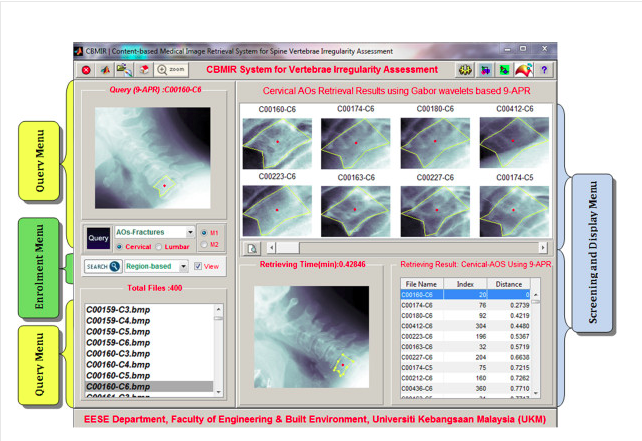
\includegraphics[scale=0.5]{imagenes/CBMIR.png}  %el parámetro scale permite agrandar o achicar la imagen. En el nombre de archivo puede especificar directorios
\label{CBMIR}
\caption{Sistema de recuperación de imágenes CBMIR}
\end{figure}

La visualización se realiza en la parte derecha de la pantalla. En la parte superior se aprecian todas las imágenes resultantes de la consulta, mientras que en la parte inferior podemos obtener mas información sobre cada una de esas imágenes.\\

Mientras que para la consulta se utiliza la parte izquierda. En ella se puede seleccionar el descriptor y la imagen a usar.\\

\subsection{Visual Clustering of Image Search Results}

La visualización de ese sistema implementado por Trystan G. Upstill, Rajehndra Nagappan y Nick Craswellb se basa a su vez en un modelo primavera desarrollado por Olsen y Korfhage. Esta técnica fue adaptada de RadViz. En este sistema, RadViz, los puntos de referencia se distribuyen en torno de un círculo, mientras que los elementos de datos están distribuidos en el círculo según su atracción a los puntos de referencia.\\

En esta imagen se puede apreciar lo explicado:\\

\begin{figure}[H] %con el [H] le obligamos a situar aquí la figura
\centering
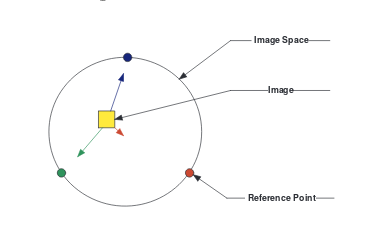
\includegraphics[scale=0.7]{imagenes/VCISR.png}  %el parámetro scale permite agrandar o achicar la imagen. En el nombre de archivo puede especificar directorios
\label{VCISR}
\caption{Puntos de atracción VCISR}
\end{figure}

Ahora veamos la representanción visual de una salida producida por una consulta.\\

\begin{figure}[H] %con el [H] le obligamos a situar aquí la figura
\centering
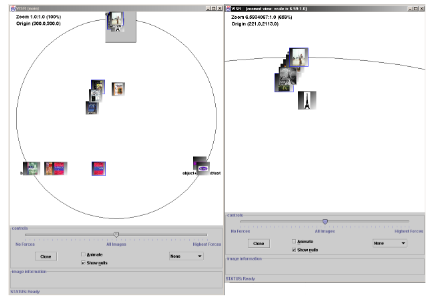
\includegraphics[scale=0.7]{imagenes/VCISR2.png}  %el parámetro scale permite agrandar o achicar la imagen. En el nombre de archivo puede especificar directorios
\label{VCISR}
\caption{Salida VCISR}
\end{figure}

Podemos apreciar como se distribuyen las imágenes a lo largo del círculo siguiendo el patrón comentado anteriormente.\\

Por otro lado podemos ver lo que ocurre al hacer zoom sobre una región. Al hacerlo apreciamos nuevas imágenes que permanecían ocultas.\\


\section{Fundamentos}

Este trabajo se basa en un sistema de recuperación de imágenes existente llamado \textit{Java Multimedia Retrival}, \textit{JMR}. Se trata de un \textit{CBIR} de código libre cuyo desarrollador principal e impulsor es el profesor Jesús Chamorro Martínez del departamento de Ciencias de la Computación e Inteligencia Artificial de la Universidad de Granada.\\

Se va hablar durante esta memoria sobre el espacio de color, por lo que es necesario darle una definición para saber a que nos referimos concretamente.\\

Por espacio de color nos referimos a un sistema de interpretación de color, una manera específica estructurar los colores de una imagen o vídeo. También es necesario hablar sobre los modelos de color, que se tratan de modelos matemáticos abstractos que describen la forma en la que cual los colores pueden ser representados como tuplas de números, normalmente como tres o cuatro valores o componentes de color, un ejemplo de esto sería RGB, en el que un color se descompone en tres valores, el valor de rojo, verde y azul.\\


\begin{figure}[H] %con el [H] le obligamos a situar aquí la figura
\centering
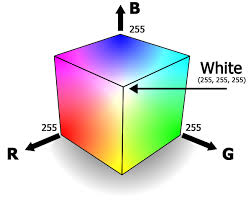
\includegraphics[scale=0.7]{imagenes/rgb.jpeg}  %el parámetro scale permite agrandar o achicar la imagen. En el nombre de archivo puede especificar directorios
\label{rgb.jpeg}
\caption{Modelo de color RGB}
\end{figure}

Otro ejemplo de espacio de color sería el \textit{HMMD}. Este espacio de color (Hue-Max-Min-Diff), es cercano a un espacio de color perceptualmente uniforme. Los nombres componentes, correspondientes a los distintos nombres, se pueden calcular a partir de RGB siguiente las siguientes transformaciones:

\begin{itemize}
\item \textbf{Max}: máximo(R,G,B)
\item \textbf{Min}: mínimo(R,G,B)
\item \textbf{Diff}: Max-min
\end{itemize}

Por otro lado, incluso se puede definir otro componente, llamado \texbf{Sum} = (Max+Min)/2.\\

En total habría una cantidad de 5 componentes en este espacio de color. Sin embargo, un cojunto de 3 elementos, {H,Max,Min} o {H,Diff,Sum}, es suficiente para para formar este espacio de color y especificar un punto de color.\\

\textit{Hue}, tiene la misma propiedad que su equivalente en el espacio de color HSV. \text{Hue} se mueve en el rango [0º, 360º]. \textit{Max} se mueve en el rango [0,1] y especifica cuanto color negro se encuentra presente, dando la sensación de sombra u oscuridad. \textit{Min}, rango [0,1], especifica cuanto color blanco se encuentra presente, dando la sensación de blanqueado. \textit{Diff}, rango [0,1], especifica como de cercano es un color a los colores puros, dando la sensación de tono o colorido. Finalmente, \textit{Sum}, especifica el brillo del color.
 
\begin{figure}[H] %con el [H] le obligamos a situar aquí la figura
\centering
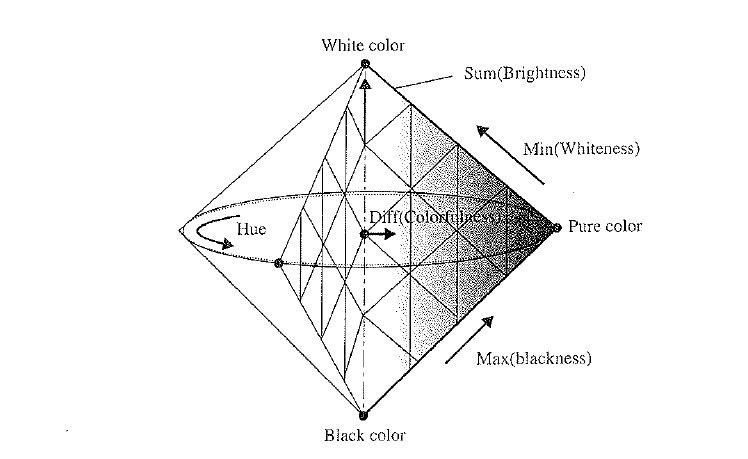
\includegraphics[scale=0.7]{imagenes/hmmd1.jpg}  %el parámetro scale permite agrandar o achicar la imagen. En el nombre de archivo puede especificar directorios
\label{hmmd1.jpg}
\caption{Modelo de color HMMD}
\end{figure}

\begin{figure}[H] %con el [H] le obligamos a situar aquí la figura
\centering
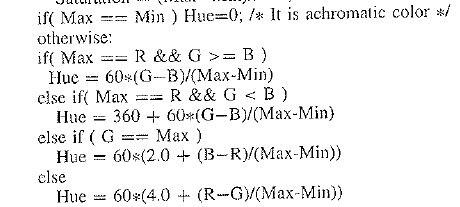
\includegraphics[scale=0.7]{imagenes/hmmd2.jpg}  %el parámetro scale permite agrandar o achicar la imagen. En el nombre de archivo puede especificar directorios
\label{hmmd2.jpg}
\caption{Cálculo Hue HMMD}
\end{figure}


Para este proyecto van a ser implementados una serie de descriptores. Estos descriptores se corresponden al tipo información general, previamente comentado, concretamente sobre el color. Estos son:

\begin{itemize}

\item Single Color Descriptor

\item MPEG7ColorStructure

\end{itemize}

\subsection{Single Color Descriptor}

Este descriptor de color se basa en el color medio de la imagen. Para calcularlo recorre una imagen en el espacio de color RGB píxel a píxel, obteniendo sus valores R, G y B. Cuando termina de recorrer todos los píxeles, calcula el color medio.

\subsection{MPEG7ColorStructure}

MPEG7ColorStructure es un descriptor de color que captura el contenido del color (similar a un histograma del color) e información sobre la estructura de este contenido. Su principal funcionalidad es la comparación imagen-imagen y se usa en la recuperación de imágenes, donde puede consistir una imagen de un solo marco rectangular o de forma arbitraria, posiblemente desconectado, regiones. El método de extracción incrusta información de estructura de color en el descriptor teniendo en cuenta todos los colores en un elemento estructurado de 8x8 píxeles que se desliza sobre la imagen, en lugar de considerar cada píxel por separado. A diferencia del histograma de color, este descriptor puede distinguir entre dos imágenes en las que un determinado color está presente en cantidades idénticas pero donde la estructura de los grupos de píxeles que tienen ese color es diferente en las dos imágenes. Los valores de color son dados por el ColorSpace MMD que se cuantifica de forma no uniforme en \textit{bin}, recipientes, de tamaño 32, 64, 128 o 256. Cada valor de amplitud de \textit{bin} está representado por un código de 8 bits. Este descriptor proporciona funcionalidad adicional y rendimiento en la recuperación de imágenes, basado en la similitud similitud, prsentando una mejora en comparación con el histograma de color ordinario.

\section{Objetivos}

Como todo proyecto que se realiza, este ha de tener una serie de objetivos que justifiquen su elaboración. Por lo que en este apartado se van a discutir los objetivos de este, dividiéndose en objetivos principales y secundarios.\\

Los principales, son los objetivos que el proyecto debe cumplir completamente. Mientras que los secundarios son objetivos que el proyecto no debe cumplir íntegramente, pero que en caso de hacerlo, suponen un gran valor añadido al proyecto. Cabe destacar que en este caso, los objetivos secundarios han sido satisfechos en su totalidad.\\

\subsection{Objetivos principales}

\begin{itemize}
  \item Desarrollar un sistema de recuperación de imágenes para plataformas móviles, para la plataforma Android concretamente. Actualmente el número de CBIR no es muy grande y no son muy conocidos por los usuarios, por lo que puede verse como una gran oportunidad.
  
  \item Este sistema debe ser capaz de permitir al usuario elegir la imagen consulta de su galería, o mediante la cámara del dispositivo, permitiendo realizar la consulta con dichas imágenes.
  
  \item Los resultados deben ser obtenidos en un periodo de tiempo aceptable. Esto ha de ser así, ya que en caso contrario, la experiencia del usuario se resentiría, lo que podría traducirse en un abandono de la aplicación.  
\end{itemize}


\subsection{Objetivos secundarios}

Una vez desarrollados los principales objetivos del proyecto, se explicarán los secundarios:

\begin{itemize}
  \item Utilizar una base de datos para almacenar los resultados. De esta manera, una vez calculada la primera consulta, el tiempo del resto se reduce drásticamente, lo que se traduce en una mejor experiencia para el usuario.

  \item Permitir al usuario modificar ajustes de la consulta. Logrando esto, el usuario puede adecuar la consulta a sus necesidades concretas, mejorando su experiencia con la aplicación.
\end{itemize}

%
\chapter{Objetivos}
\label{cap:objetivos}

Como todo proyecto que se realiza, este ha de tener una serie de objetivos que justifiquen su realización. Por lo que en este apartado se van a discutir los objetivos de este, diviendose en objetivos principales y secundarios.\\

Los principales son los objetivos que el proyecto debe cumplir completamente, mientras que los secundarios son objetivos que el proyecto no debe cumplir integramente, pero que en caso de cumplirlos, suponen un gran valor añadido al proyecto. Cabe destacar que en este caso, los objetivos secundarios han sido satisfechos en su totalidad.\\

\section{Objetivos principales}

\begin{itemize}
  \item Desarrollar un sistema de recuperación de imágenes para plataformas móviles, para la plataforma Android concretamente. Actualmente el número de CBIR no es muy grande y no son muy conocidos por los usuarios, por lo que puede verse como una gran oportunidad.
  
  \item Este sistema debe ser capaz de permitir al usuario elegir la imagen consulta de su galería, o mediante la cámara del dispositivo, permitiendo realizar la consulta con dichas imágenes.
  
  \item Los resultados deben ser obtenidos en un periodo de tiempo aceptable. Esto ha de ser así, ya que en caso contrario, la experiencia del usuario se resintiría, lo que podría traducirse en un abandono de la aplicación.  
  
\end{itemize}


\section{Objetivos secundarios}

Una vez desarrollados los principales objetivos del proyecto, se explicarán los secundarios:

\begin{itemize}
  \item Utilizar una base de datos para almacenar los resultados. De esta manera, una vez calculada la primera consulta, el tiempo del resto se reduce drásticamente, lo que se traduce en una mejor experiencia para el usuario.

  \item Permitir al usuario modificar ajustes de la consulta. Logrando esto, el usuario puede adecuar la consulta a sus necesidades concretas, mejorando su experiencia con la aplicación.
\end{itemize}

%
%\chapter{Análisis}
\label{cap:analisis}

\section{Introducción al problema}

Nos encontramos ante la siguiente situación: Debemos permitir al usuario realizar consultas sobre las imágenes de su dispositivo, tomando como imagen consulta la obtenida desde la cámara o desde la galería.\\

Los valores proporcionados por cada descriptor se encuentran en el rango 0-1. Los cálculos para determinar la posición se realizarán con esos datos. Para ello, se colocarán de izquierda a derecha, formando un total de 4 columnas, siguiendo un orden lógico y natural que es entendido rápida y claramente por el usuario.\\

Dado el número de imágenes y el tamaño de pantalla de los dispositivos, no todas podrán ser vistas a la vez ni, por lo que el usuario debe ser capaz de desplazarse por las imágenes resultado contando con guı́as que le indiquen el orden de las diferentes imágenes mostradas.\\

También deberá ser posible obtener información de las imágenes mostradas con el fin de comprender mejor la visualización y su vez comprobar el correcto funcionamiento de los descriptores.\\

El proyecto está pensado por el momento sólo para smartphones, debido a falta de medios, por lo que la posibilidad de girar pantalla ha sido desactivada. Como trabajo futuro, se realizarán los cambios oportunos para que pueda ser utilizado en tablets.

\section{Especificación de requisitos}

Por requisitos podemos entender: Condición o capacidad que necesita el usuario para resolver un problema o conseguir un objetivo determinado.\\

Como en todo proyecto de software, los requisitos deben ser especificados antes de empezar el desarrollo del mismo.\\

En esta sección vamos a detallar cada uno de los distintos requisitos necesitados agrupados en requisitos funcionales, no funcionales y de información.\\

\subsection{Requisitos funcionales}

Los requisitos funcionales se encargan de especificar cómo se realizará la interacción entre el sistema y su entorno, indicando los servicios que ha de tener el sistema o cómo responderá ante ciertos estímulos.\\

Este proyecto cuenta con los siguientes requisitos funcionales:\\

\textbf{RF-1. Imágenes:} Gestión de imágenes.\\
 
   RF-1.1. Se debe permitir cargar cualquier imagen desde cámara o galería como imagen consulta.
   
   RF-1.2. Se debe permitir cargar cualquier número de imágenes para su consulta.
   
   RF-1.3. La elección de la imagen consulta ha de ser sencilla.\\
   
\textbf{RF-2. Descriptores:} Gestión de descriptores.\\    
   
   RF-2.1. Ha de ser posible la elección de cualquier descriptor disponible.
      
   RF-2.2. La consulta ha de realizarse con únicamente con el descriptor seleccionado.\\    
   
\textbf{RF-3. Base de datos:} Gestión de base de datos.\\    
   
   RF-3.1. El usuario debe poder precalcular la base de datos antes de realizar cualquier consulta.
   
   RF-3.2. El usuario debe poder eliminar la base de datos, en caso de que lo considere necesario.\\

\textbf{RF-4 Interacción} Gestión de la interacción.\\

   RF-4.1. El usuario debe poder interactuar a través de la pantalla.
   
   RF-4.2. El usuario debe ser capaz de desplazar las imágenes consulta de izquierda a derecha y viceversa.
   
   RF-4.3. El usuario debe ser capaz de desplazar las imágenes resultado de arriba hacia abajo y viceversa.
   
   RF-4.4. El usuario debe poder ver las imágenes a tamaño real al pulsar sobre ellas.

\textbf{RF-5 Información adicional} Gestión de la información adicional.\\

   RF-5.1. El usuario debe poder consultar información sobre el desarrollo del proyecto.
   
   RF-5.2. El usuario debe ser capaz de obtener más información sobre sistemas de recuperación de imágenes y sobre los descriptores.
   
           
\subsection{Requisitos no funcionales}
Los requisitos no funcionales describen cualidades o restricciones del sistema que no se relacionan de forma directa con el comportamiento funcional del mismo.

Este proyecto cuenta con los siguientes requisitos no funcionales:\\

\textbf{RNF-1} Debe de utilizar la mínima cantidad de memoria posible.

\textbf{RNF-2} Ha de ser implementando en Android.

\textbf{RNF-3} Ha de requerir los permisos mínimos para funcionar.

\textbf{RNF-4} Las consultas se realizan utilizando una única imagen consulta.
   
\textbf{RNF-5} El tamaño de las imágenes mostradas ha de ser lo suficientemente grande para poder verse correctamente.

\textbf{RNF-6} Se debe indicar el orden en el que fueron dibujadas las imágenes.\\

\subsection{Requisitos de información}

Este tipo de requisito de detallar la necesidad por parte del sistema del almacenamiento de la información. \\

\textbf{RI-1} Almacenar información de la consulta para evitar nuevas cálculos innecesarias.


\section{Historias de usuario}

Cuando nos referimos a historias de usuario, nos refererimos a la representación de un requisito software que se encuentra escrito en varias frases cortas, utilizando el lenguaje común del usuario. Esto facilita la comprensión y realización de los requisitos de un proyecto. Se trata de otra manera de ver los requisitos software que se acaban de explicar. Por lo que vamos a ver sólo los pricipales\\

\begin{table}[H]
	\begin{center}
		\begin{tabular} {l|c|l}
			\hline
			1 & \multicolumn{2}{c}{Interacción con la interfaz} \\ \noalign{\hrule height 1pt}
			\multicolumn{3}{l}{Descripción} \\ \hline
			\multicolumn{3}{p{12cm}}{Se podra mover con libertad por los distintos menús diponibles en la interfaz.} \\ \noalign{\hrule height 1pt}
			\multicolumn{3}{l}{Pruebas de aceptación} \\ \hline
			\multicolumn{3}{p{12cm}}{ - Comprobar que al pulsar en al pulsar el item \textbf{consulta} se muestra la interfaz asociada.} \\
			\multicolumn{3}{p{12cm}}{ - Comprobar que al pulsar en el action button, este se despliega mostrando dos opciones, cámara y galería.} \\
			\multicolumn{3}{p{12cm}}{ - Comprobar que al pulsar en al pulsar el item \textbf{ajustes} se muestra la interfaz asociada.} \\ \hline
			\multicolumn{3}{p{12cm}}{ - Comprobar que al pulsar en al pulsar el item \textbf{adicional} se muestra la interfaz asociada.} \\ 
			\hline
		\end{tabular}
	\end{center}
	\caption{Historia de usuario - Interacción con la interfaz}
	\label{tab:interaccion-interfaz}
\end{table}

\begin{table}[H]
	\begin{center}
		\begin{tabular} {l|c|l}
			\hline
			2 & \multicolumn{2}{c}{Cargar imagen cámara} \\ \noalign{\hrule height 1pt}
			\multicolumn{3}{l}{Descripción} \\ \hline
			\multicolumn{3}{p{12cm}}{Se podra mover cargar la imagen consulta utilizando la cámara del dispositivo.} \\ \noalign{\hrule height 1pt}
			\multicolumn{3}{l}{Pruebas de aceptación} \\ \hline
			\multicolumn{3}{p{12cm}}{ - Comprobar que al pulsar en al pulsar el item \textbf{cámara} del \textit{floating button}, se lanza la actividad cámara, pudiendo elegir la delantera o trasera en caso de que se diponga de ellas.} \\
			\multicolumn{3}{p{12cm}}{ - Comprobar que al tomar una fotografía esta se añade a la sección de imágenes consulta.} \\
			\multicolumn{3}{p{12cm}}{ - Comprobar que al pulsar en al pulsar en el item \textbf{consultar}, se realiza la consulta con esta nueva imagen.} \\ \hline
		\end{tabular}
	\end{center}
	\caption{Historia de usuario - Cargar imagen consulta cámara}
	\label{tab:interaccion-interfaz}
\end{table}

\begin{table}[H]
	\begin{center}
		\begin{tabular} {l|c|l}
			\hline
			3 & \multicolumn{2}{c}{Cargar imagen galería} \\ \noalign{\hrule height 1pt}
			\multicolumn{3}{l}{Descripción} \\ \hline
			\multicolumn{3}{p{12cm}}{Se podra cargar la imagen consulta utilizando la galería del dispositivo.} \\ \noalign{\hrule height 1pt}
			\multicolumn{3}{l}{Pruebas de aceptación} \\ \hline
			\multicolumn{3}{p{12cm}}{ - Comprobar que al pulsar en al pulsar el item \textbf{galería} del \textit{floating button}, se lanza la galería.} \\
			\multicolumn{3}{p{12cm}}{ - Comprobar que al tomar seleccionar una imagen, esta se añade a la sección de imágenes consulta.} \\
			\multicolumn{3}{p{12cm}}{ - Comprobar que al pulsar en al pulsar en el item \textbf{consultar}, se realiza la consulta con esta nueva imagen.} \\ \hline
		\end{tabular}
	\end{center}
	\caption{Historia de usuario - Cargar imagen consulta galería}
	\label{tab:interaccion-interfaz}
\end{table}


\begin{table}[H]
	\begin{center}
		\begin{tabular} {l|c|l}
			\hline
			4 & \multicolumn{2}{c}{Cambiar de descriptor} \\ \noalign{\hrule height 1pt}
			\multicolumn{3}{l}{Descripción} \\ \hline
			\multicolumn{3}{p{12cm}}{Se podra cambiar el descriptor que se emplea durante las consultas.} \\ \noalign{\hrule height 1pt}
			\multicolumn{3}{l}{Pruebas de aceptación} \\ \hline
			\multicolumn{3}{p{12cm}}{ - Comprobar que al pulsar sobre el descriptor deseado este queda maracado como activo.} \\
			\multicolumn{3}{p{12cm}}{ - Comprobar que solo un descriptor puede ser seleccionado.} \\
			\multicolumn{3}{p{12cm}}{ - Comprobar que al pulsar en al pulsar en el item \textbf{consultar}, se realiza la consulta con este descriptor seleccionado.} \\ \hline
		\end{tabular}
	\end{center}
	\caption{Historia de usuario - Cambiar descriptor}
	\label{tab:interaccion-interfaz}
\end{table}

\begin{table}[H]
	\begin{center}
		\begin{tabular} {l|c|l}
			\hline
			5 & \multicolumn{2}{c}{Eliminar base de datos} \\ \noalign{\hrule height 1pt}
			\multicolumn{3}{l}{Descripción} \\ \hline
			\multicolumn{3}{p{12cm}}{Se podra eliminar la base de datos.} \\ \noalign{\hrule height 1pt}
			\multicolumn{3}{l}{Pruebas de aceptación} \\ \hline
			\multicolumn{3}{p{12cm}}{ - Comprobar que al pulsar sobre la opción \textit{Eliminar BD} se lanza un desplegable para realizar la acción.} \\
			\multicolumn{3}{p{12cm}}{ - Comprobar que al pulsar en aceptar, se notifica de que la BD ha sido eliminada.} \\
		\end{tabular}
	\end{center}
	\caption{Historia de usuario - Eliminar base de datos}
	\label{tab:interaccion-interfaz}
\end{table}

\begin{table}[H]
	\begin{center}
		\begin{tabular} {l|c|l}
			\hline
			6 & \multicolumn{2}{c}{Calcular base de datos} \\ \noalign{\hrule height 1pt}
			\multicolumn{3}{l}{Descripción} \\ \hline
			\multicolumn{3}{p{12cm}}{Se podra precalcular la base de datos para agilizar consultas.} \\ \noalign{\hrule height 1pt}
			\multicolumn{3}{l}{Pruebas de aceptación} \\ \hline
			\multicolumn{3}{p{12cm}}{ - Comprobar que al pulsar sobre la opción \textit{Calcular BD} se lanza un diálogo sobre el proceso.} \\
			\multicolumn{3}{p{12cm}}{ - Comprobar que al realizar una consulta, el tiempo es menor que si no hubiese base de datos.} \\
		\end{tabular}
	\end{center}
	\caption{Historia de usuario - Calcular base de datos}
	\label{tab:interaccion-interfaz}
\end{table}

\begin{table}[H]
	\begin{center}
		\begin{tabular} {l|c|l}
			\hline
			7 & \multicolumn{2}{c}{Elegir número de imágenes} \\ \noalign{\hrule height 1pt}
			\multicolumn{3}{l}{Descripción} \\ \hline
			\multicolumn{3}{p{12cm}}{Se podra elegir el número de imágenes que serán consultadas.} \\ \noalign{\hrule height 1pt}
			\multicolumn{3}{l}{Pruebas de aceptación} \\ \hline
			\multicolumn{3}{p{12cm}}{ - Comprobar que al pulsar sobre la opción \textit{Elegir número de imagenes} se lanza un desplegable permitiendonos elegir el número.} \\
			\multicolumn{3}{p{12cm}}{ - Comprobar que el número de las imágenes resultado se corresponde con el establecido previamente.} \\
		\end{tabular}
	\end{center}
	\caption{Historia de usuario - Elegir número de imágenes}
	\label{tab:interaccion-interfaz}
\end{table}

\begin{table}[H]
	\begin{center}
		\begin{tabular} {l|c|l}
			\hline
			8 & \multicolumn{2}{c}{Interactuar con las imágenes consulta} \\ \noalign{\hrule height 1pt}
			\multicolumn{3}{l}{Descripción} \\ \hline
			\multicolumn{3}{p{12cm}}{Se podra interactuar con las imágenes consulta.} \\ \noalign{\hrule height 1pt}
			\multicolumn{3}{l}{Pruebas de aceptación} \\ \hline
			\multicolumn{3}{p{12cm}}{ - Comprobar que se puede realizar movimiento scroll de derecha a izquierda y viceversa sobre las imágenes consulta, siempre que haya las suficientes.} \\
			\multicolumn{3}{p{12cm}}{ - Comprobar que al pulsar sobre una, esta se muestra a pantalla completa indicándonos la posición que ocupa respecto a las demás.} \\
		\end{tabular}
	\end{center}
	\caption{Historia de usuario - Interactuar con las imágenes consulta }
	\label{tab:interaccion-interfaz}
\end{table}

\begin{table}[H]
	\begin{center}
		\begin{tabular} {l|c|l}
			\hline
			9 & \multicolumn{2}{c}{Interactuar con las imágenes resultado} \\ \noalign{\hrule height 1pt}
			\multicolumn{3}{l}{Descripción} \\ \hline
			\multicolumn{3}{p{12cm}}{Se podra interactuar con las imágenes resultado.} \\ \noalign{\hrule height 1pt}
			\multicolumn{3}{l}{Pruebas de aceptación} \\ \hline
			\multicolumn{3}{p{12cm}}{ - Comprobar que se puede realizar movimiento scroll hacia arriba, hacia abajo y viceversa sobre las imágenes resultado, siempre que haya las suficientes.} \\
			\multicolumn{3}{p{12cm}}{ - Comprobar que al pulsar sobre una, esta se muestra a pantalla completa indicándonos la posición que ocupa respecto a las demás, y la distancia respecto a la imagen consulta.} \\
		\end{tabular}
	\end{center}
	\caption{Historia de usuario - Interactuar con las imágenes consulta}
	\label{tab:interaccion-interfaz}
\end{table}

\section{Diagramas de secuencia}

Establecidas las historias de usuario, procedamos con los diagramas de secuencia. Estos se usan para establecer el modo en que interaccionan objetos en un sistema atendiendo a UML.

\begin{figure}[H] %con el [H] le obligamos a situar aquí la figura
\centering
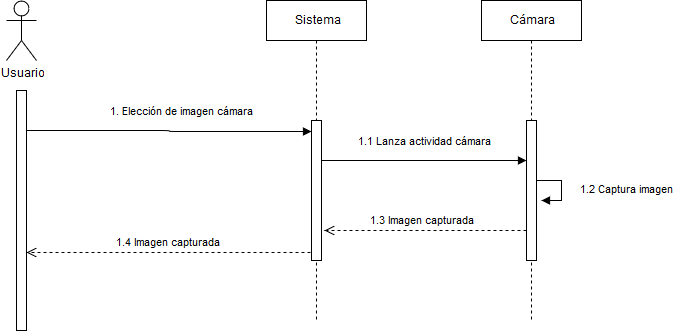
\includegraphics[scale=0.6]{imagenes/imagenCamara.png}  %el parámetro scale permite agrandar o achicar la imagen. En el nombre de archivo puede especificar directorios
\label{imagenCamara.png}
\caption{Diagrama de secuencia imagen consulta cámara}
\end{figure}

\begin{figure}[H] %con el [H] le obligamos a situar aquí la figura
\centering
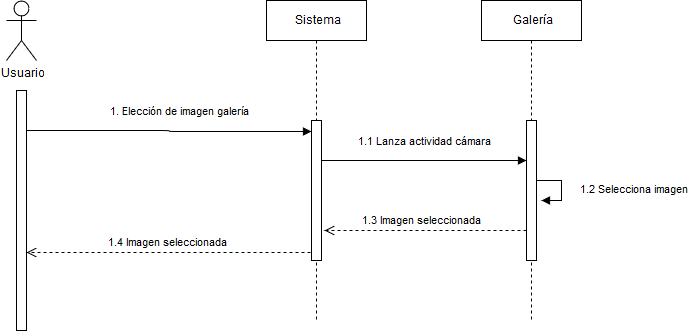
\includegraphics[scale=0.6]{imagenes/imagenGaleria.png}  %el parámetro scale permite agrandar o achicar la imagen. En el nombre de archivo puede especificar directorios
\label{imagenGaleria.png}
\caption{Diagrama de secuencia imagen consulta galería}
\end{figure}

\begin{figure}[H] %con el [H] le obligamos a situar aquí la figura
\centering
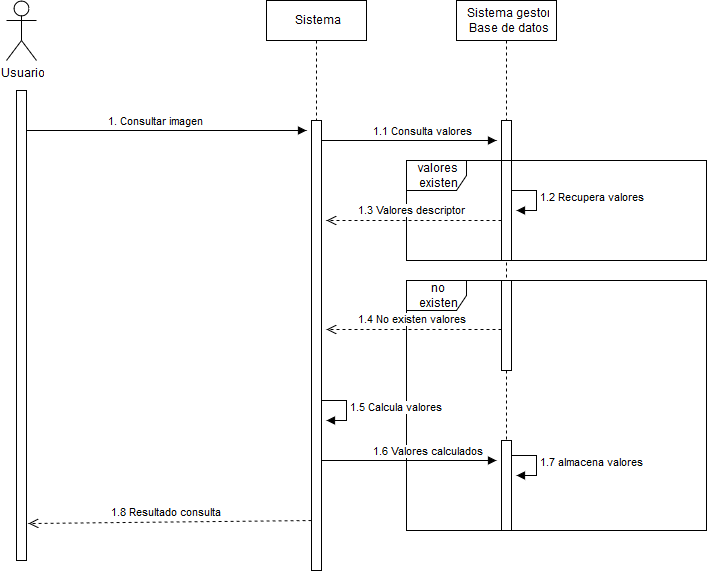
\includegraphics[scale=0.6]{imagenes/realizarConsulta.png}  %el parámetro scale permite agrandar o achicar la imagen. En el nombre de archivo puede especificar directorios
\label{realizarConsulta.png}
\caption{Diagrama de secuencia imagen realizar consulta}
\end{figure}

\begin{figure}[H] %con el [H] le obligamos a situar aquí la figura
\centering
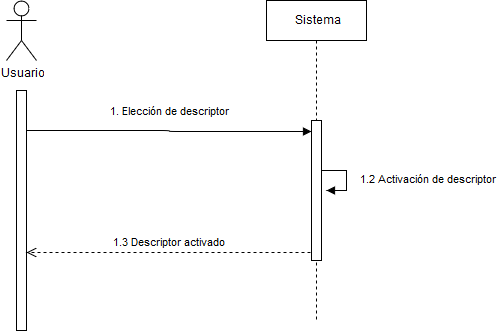
\includegraphics[scale=0.6]{imagenes/eleccionDescriptor.png}  %el parámetro scale permite agrandar o achicar la imagen. En el nombre de archivo puede especificar directorios
\label{realizarConsulta.png}
\caption{Diagrama de secuencia elección descriptor}
\end{figure}

\begin{figure}[H] %con el [H] le obligamos a situar aquí la figura
\centering
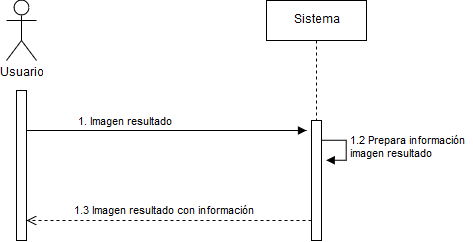
\includegraphics[scale=0.6]{imagenes/imagenResultadoInformacion.png}  %el parámetro scale permite agrandar o achicar la imagen. En el nombre de archivo puede especificar directorios
\label{imagenResultadoInformacion.png}
\caption{Diagrama de secuencia información imagen resultado}
\end{figure}

\begin{figure}[H] %con el [H] le obligamos a situar aquí la figura
\centering
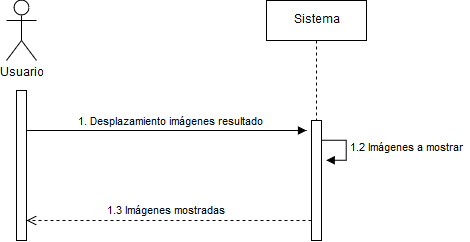
\includegraphics[scale=0.6]{imagenes/desplazamientoResultado.png}  %el parámetro scale permite agrandar o achicar la imagen. En el nombre de archivo puede especificar directorios
\label{desplazamientoResultado.png}
\caption{Diagrama de secuencia desplazamiento imagen resultado}
\end{figure}

\begin{figure}[H] %con el [H] le obligamos a situar aquí la figura
\centering
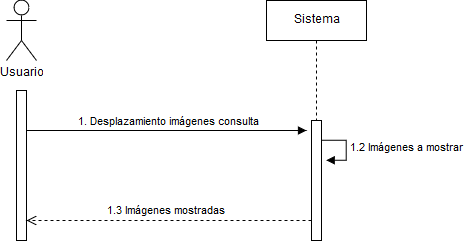
\includegraphics[scale=0.6]{imagenes/desplazamientoConsulta.png}  %el parámetro scale permite agrandar o achicar la imagen. En el nombre de archivo puede especificar directorios
\label{desplazamientoConsulta.png}
\caption{Diagrama de secuencia desplazamiento imagen consulta}
\end{figure}




%
%\chapter{Diseño}
\label{cap:diseno}

En este capítulo se va a hablar sobre el diseño del proyecto, así como de la arquitectura, herramientas y técnicas elegidas para el desarrollo del mismo.\\

El diseño es el desarrollo de aplicar una serie de métodos, técnicas y principios de diseño para traducir el modelo del análisis a una representación la cual sea posible ser codificada.\\

\section{Metodología}

La metodología seguida puede considerarse como \textit{Scrum}.\\

Al comienzo de este proyecto se tuvieron varias reuniones para establecer los objetivos y requisitos que debía de cumplir este proyecto, aunque no en demasiada profundidad, siendo esto una tarea que se llevo a cabo según lo establecido en el capítulo anterior.\\

Una vez finalizadas dichas reuniones iniciales, se establecieron una serie de fechas en las cuales se tuvieron otras reuniones para comprobar el estado del proyecto. Estas fechas coinciden con la planificación. Para cada reunión, se establecía una serie de objetivos que se debían alcanzar para el correcto desarrollo del proyecto y garantizar que se cumplía con la planificación establecida. De esta manera, se intercambiaron opiniones sobre la situación del proyecto, comentando posibles mejoras y solucionando las dudas surgidas durante las distintas etapas del desarrollo.\\

\section{Arquitectura}

El estilo arquitectónico utilizado para la realización de este proyecto ha sido el modelo vista controlador, ya que se adapta correctamente a las necesidades del sistema.
Los elementos de una arquitectura MVC son:

\begin{itemize}
\item Modelo: Es el encargado del conocimiento del dominio de la aplicación.
\item Vista: Responsable de mostrar las diferentes características del modelo al usuario.
\item Controlador: Elemento que responde a la interacción del usuario, realizando las peticiones necesarias al modelo y la vista.
\end{itemize}

Una vez definido el estilo arquitectónico se va a pasar a hablar de las herramientas que se han usado.

\section{Herramientas usadas}

En esta sección vamos a comentar las herramientas que han sido usadas durante la realización del proyecto.

\subsection{Android Studio}

Aunque no es estrictamente necesario para desarrollar aplicaciones Android, es posible utilizar eclipse por ejemplo, he decidido usarlo ya que es muy sencillo de entender y facilita al programador muchas tareas. Esto ha sido muy importante ya que, como he comentado antes, mi experiencia con Android era muy reducida.\\

Android Studio es el entorno de desarrollo integrado, \textit{IDE}, oficial para la plataforma Android. Por esta razón la documentación es abundante, lo que supone un gran punto a su favor.\\

\begin{figure}[H] %con el [H] le obligamos a situar aquí la figura
\centering
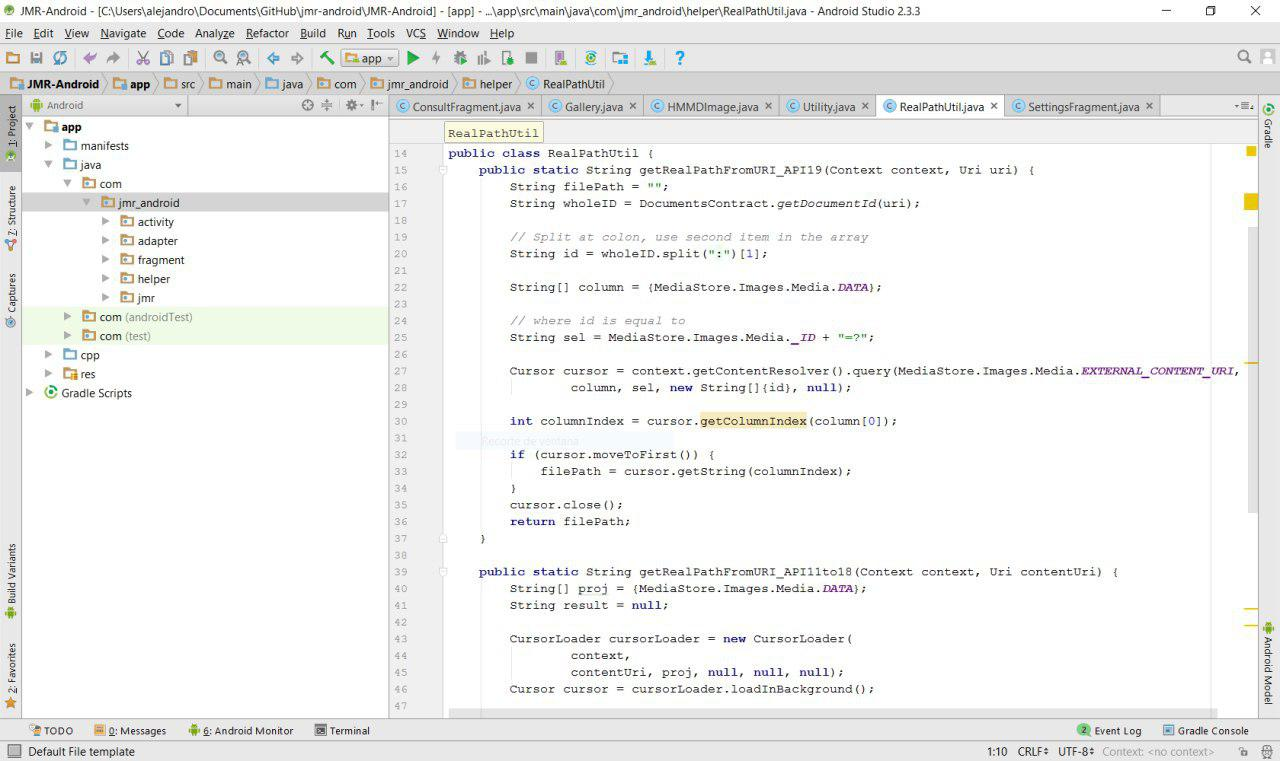
\includegraphics[scale=0.5]{imagenes/android-studio.jpg}  %el parámetro scale permite agrandar o achicar la imagen. En el nombre de archivo puede especificar directorios
\label{android-studio.jpg}
\caption{Ejemplo de proyecto Android Studio}
\end{figure}

Otra de las cosas interesantes de este \textit{IDE} es la posibilidad de diseñar interfaces de una manera muy sencilla e intuitiva, permitiendo arrastrar los elementos a las posiciones deseadas. Por lo que no se requiere un gran nivel de programación para estas tareas. Aunque si hay que comentar, que si se necesita hacer cosas más complicadas, o que no sean las estándar, si es necesario un nivel de programación avanzado, ya que en dicho caso, la ayuda proporcionada por Android Studio para estas tareas se reduce.\\ 

\subsection{Git y GitHub}

Al tratarse de un proyecto de esta magnitud, ha sido necesario utilizar una herramienta de control de versiones, como es natural se ha utilizado git.\\

También se ha usado GitHub, que se trata de un lugar donde alojar nuestros proyectos utilizando el sistema de control de versiones Git. Por lo tanto, podemos entender que git y GitHub van de la mano, al menos en este caso.\\

El repositorio del proyecto se puede consultar \href{https://github.com/acasadoquijada/jmr-android}{aquí}.

Para llevar un control del proyecto se han usado los elementos conocidos como \textit{Milestones} y \textit{Issues} por GitHub.\\

Podemos entender un \textit{Issue} como una tarea por realizar, siendo un ejemplo, \textit{seleccionar imagen de la galería}. Se les puede añadir información extra, como a que \textit{Milestone} está asociado, que persona es la encargada de solucionarlo, o se puede añadir una etiqueta para establecer el tipo.\\

\begin{figure}[H] %con el [H] le obligamos a situar aquí la figura
\centering
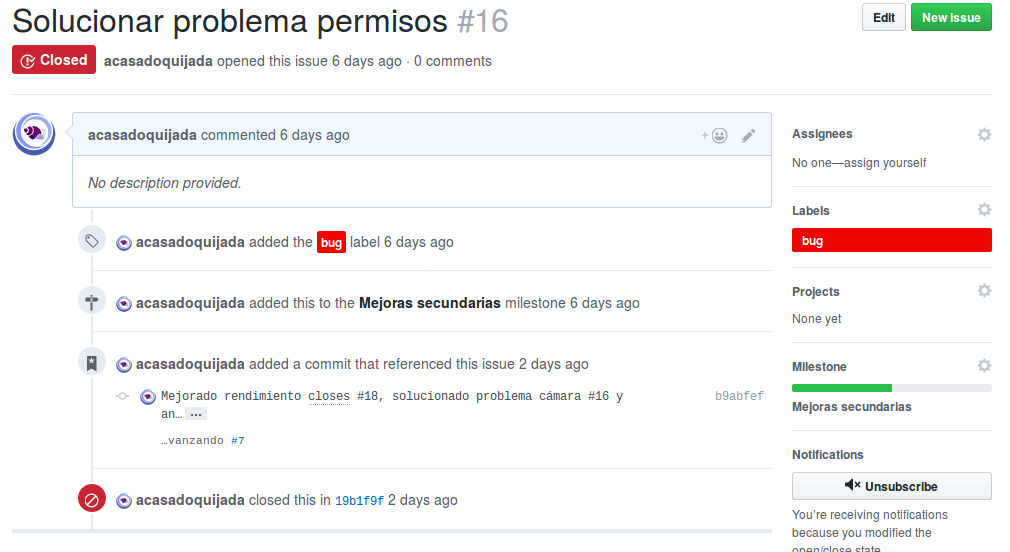
\includegraphics[scale=0.4]{imagenes/issue.png}  %el parámetro scale permite agrandar o achicar la imagen. En el nombre de archivo puede especificar directorios
\label{issue.png}
\caption{Ejemplo de issue}
\end{figure}

Por otro lado, se encuentran los \textit{Milestones}, que podemos considerarlos como hitos, es decir, un \textit{Milestone} está compuesto por varios \textit{Issues}. Por lo que también puede ser vistos como una agrupación de \textit{Issues}, una gran tarea dividida en pequeñas subtareas.\\

\begin{figure}[H] %con el [H] le obligamos a situar aquí la figura
\centering
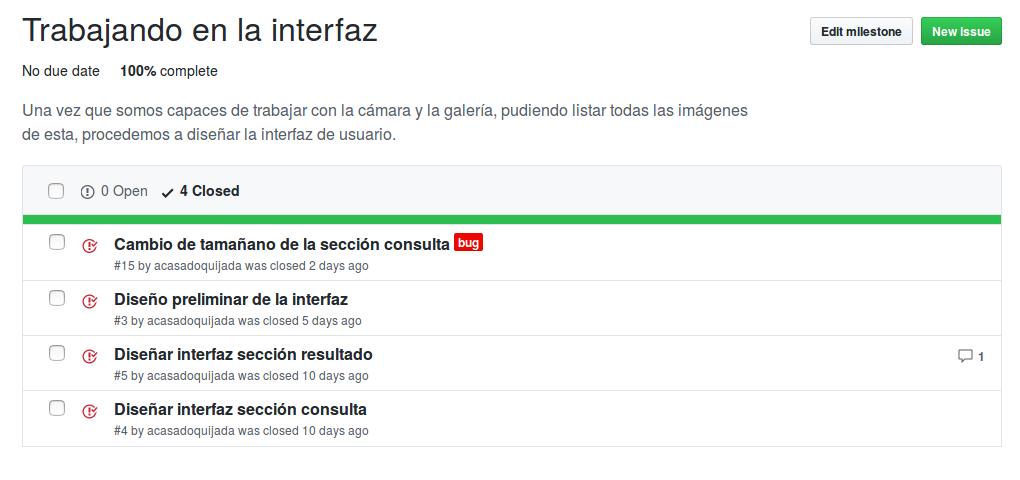
\includegraphics[scale=0.4]{imagenes/milestone.png}  %el parámetro scale permite agrandar o achicar la imagen. En el nombre de archivo puede especificar directorios
\label{milestone.png}
\caption{Ejemplo de milestone}
\end{figure}

Como se puede entender, usar ambos es de vital importancia si se desea llevar a cabo un proyecto de gran magnitud.

\subsection{Dispotivio de pruebas}

Aunque Android Studio nos ofrece la posibilidad de utilizar un emulador para lanzar la aplicación, he decidido utilizar mi dispositivo móvil, por motivos de eficiencia y comodidad. Debido a que no se podía comprobar de manera real algunos aspectos de la propia aplicación, como el consumo de memoria o el propio rendimiento de las consultas.\\

Mi smartphone es un \textit{Xiaomi redmi 4 pro}, y cuenta con las siguientes características destacables:

\begin{itemize}
\item CPU: Qualcomm Snapdragon 625, con ocho núcleos y 2GHz 
\item Memoria: 3 GB
\item Almacenamiento: 32 GB
\end{itemize}

Se tratan de unas características que suelen ser habituales de encontrar en los smartphones actuales, por lo que ha sido un gran sujeto de pruebas.

\section{Tecnicas}

Para programar en Android se utiliza \textit{Java} para la lógica, y \textit{XML} para las interfaces de usuario.\\

Como es habitual, el desarrollo en Java ha seguido un paradigma de programación orientada a objetos, \textit{POO}. En el que se han desarrollado una serie de clases que se han organizado en distintos paquetes. Esto será explicado posteriormente.\\ 

Comentar que se ha utilizado también \textit{Android NDK}. Se trata de un conjunto de herramientas que nos permiten implementar partes de la aplicación en código nativo, como \textit{C} o \textit{C++}. Esta opción es perfecta para usar en los cálculos que realiza la aplicación. Como en el caso anterior se comentará con más detalle en su correspondiente sección.\\

\begin{figure}[H] %con el [H] le obligamos a situar aquí la figura
\centering
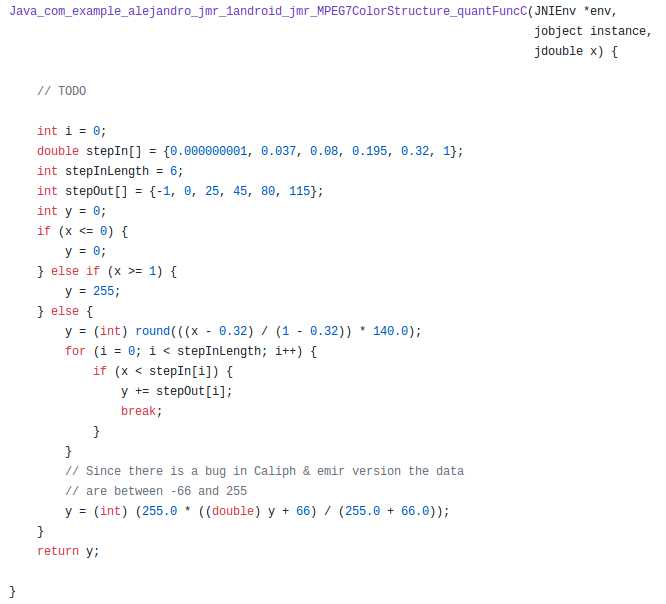
\includegraphics[scale=0.6]{imagenes/ndk.png}  %el parámetro scale permite agrandar o achicar la imagen. En el nombre de archivo puede especificar directorios
\label{ndk.png}
\caption{Ejemplo de código Android ndk}
\end{figure}

Por último comentar que se ha usado \textit{XML} para las interfaces de usuario, la mayor parte del tiempo apoyándose en el soporte proporcionado por Android Studio, pero que a la hora de realizar cosas mas complejas se ha tenido que escribir manualmente dicho código XML.

\begin{figure}[H] %con el [H] le obligamos a situar aquí la figura
\centering
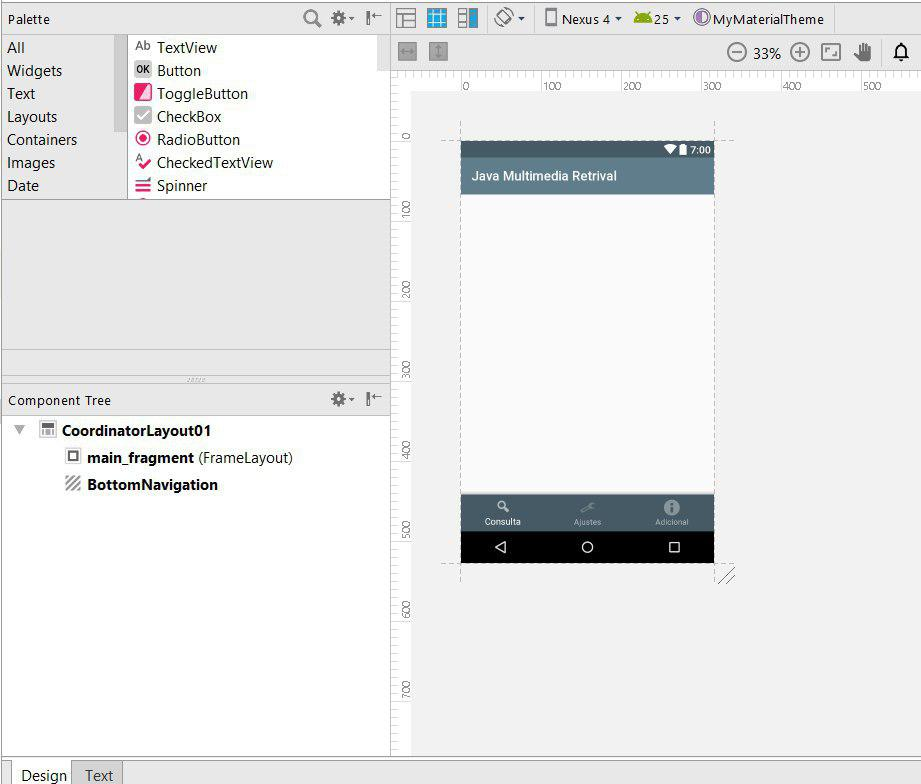
\includegraphics[scale=0.6]{imagenes/interfaz-android-studio.jpg}  %el parámetro scale permite agrandar o achicar la imagen. En el nombre de archivo puede especificar directorios
\label{interfaz-android-studio.jpg}
\caption{Ejemplo de proyecto Android Studio}
\end{figure}



%
%\input{capitulos/06_Implementacion}
%
%\input{capitulos/07_Pruebas}
%
%\input{capitulos/08_Conclusiones_y_trabajos_futuros}
%
%%\chapter{Conclusiones y Trabajos Futuros}
%
%
\nocite{*}
\bibliography{bibliografia/bibliografia}\addcontentsline{toc}{chapter}{Bibliografía}
\bibliographystyle{plain}
%
\appendix
%\chapter{Manual de usuario}
\label{cap:Manual de usuario}

\section{Permisos}

Para el correcto funcionamiento de la aplicación es necesario que el usuario de permisos a la aplicación para poder acceder tanto a la cámara, como a las imágenes del dispositivo.\\

Al iniciar la aplicación se nos pedirá permiso para acceder al contenido del teléfono, ya que es en ese instante, cuando se inicia la aplicación, el momento en el que se listan todas las imágenes del dispositivo.

\begin{figure}[H] %con el [H] le obligamos a situar aquí la figura
\centering
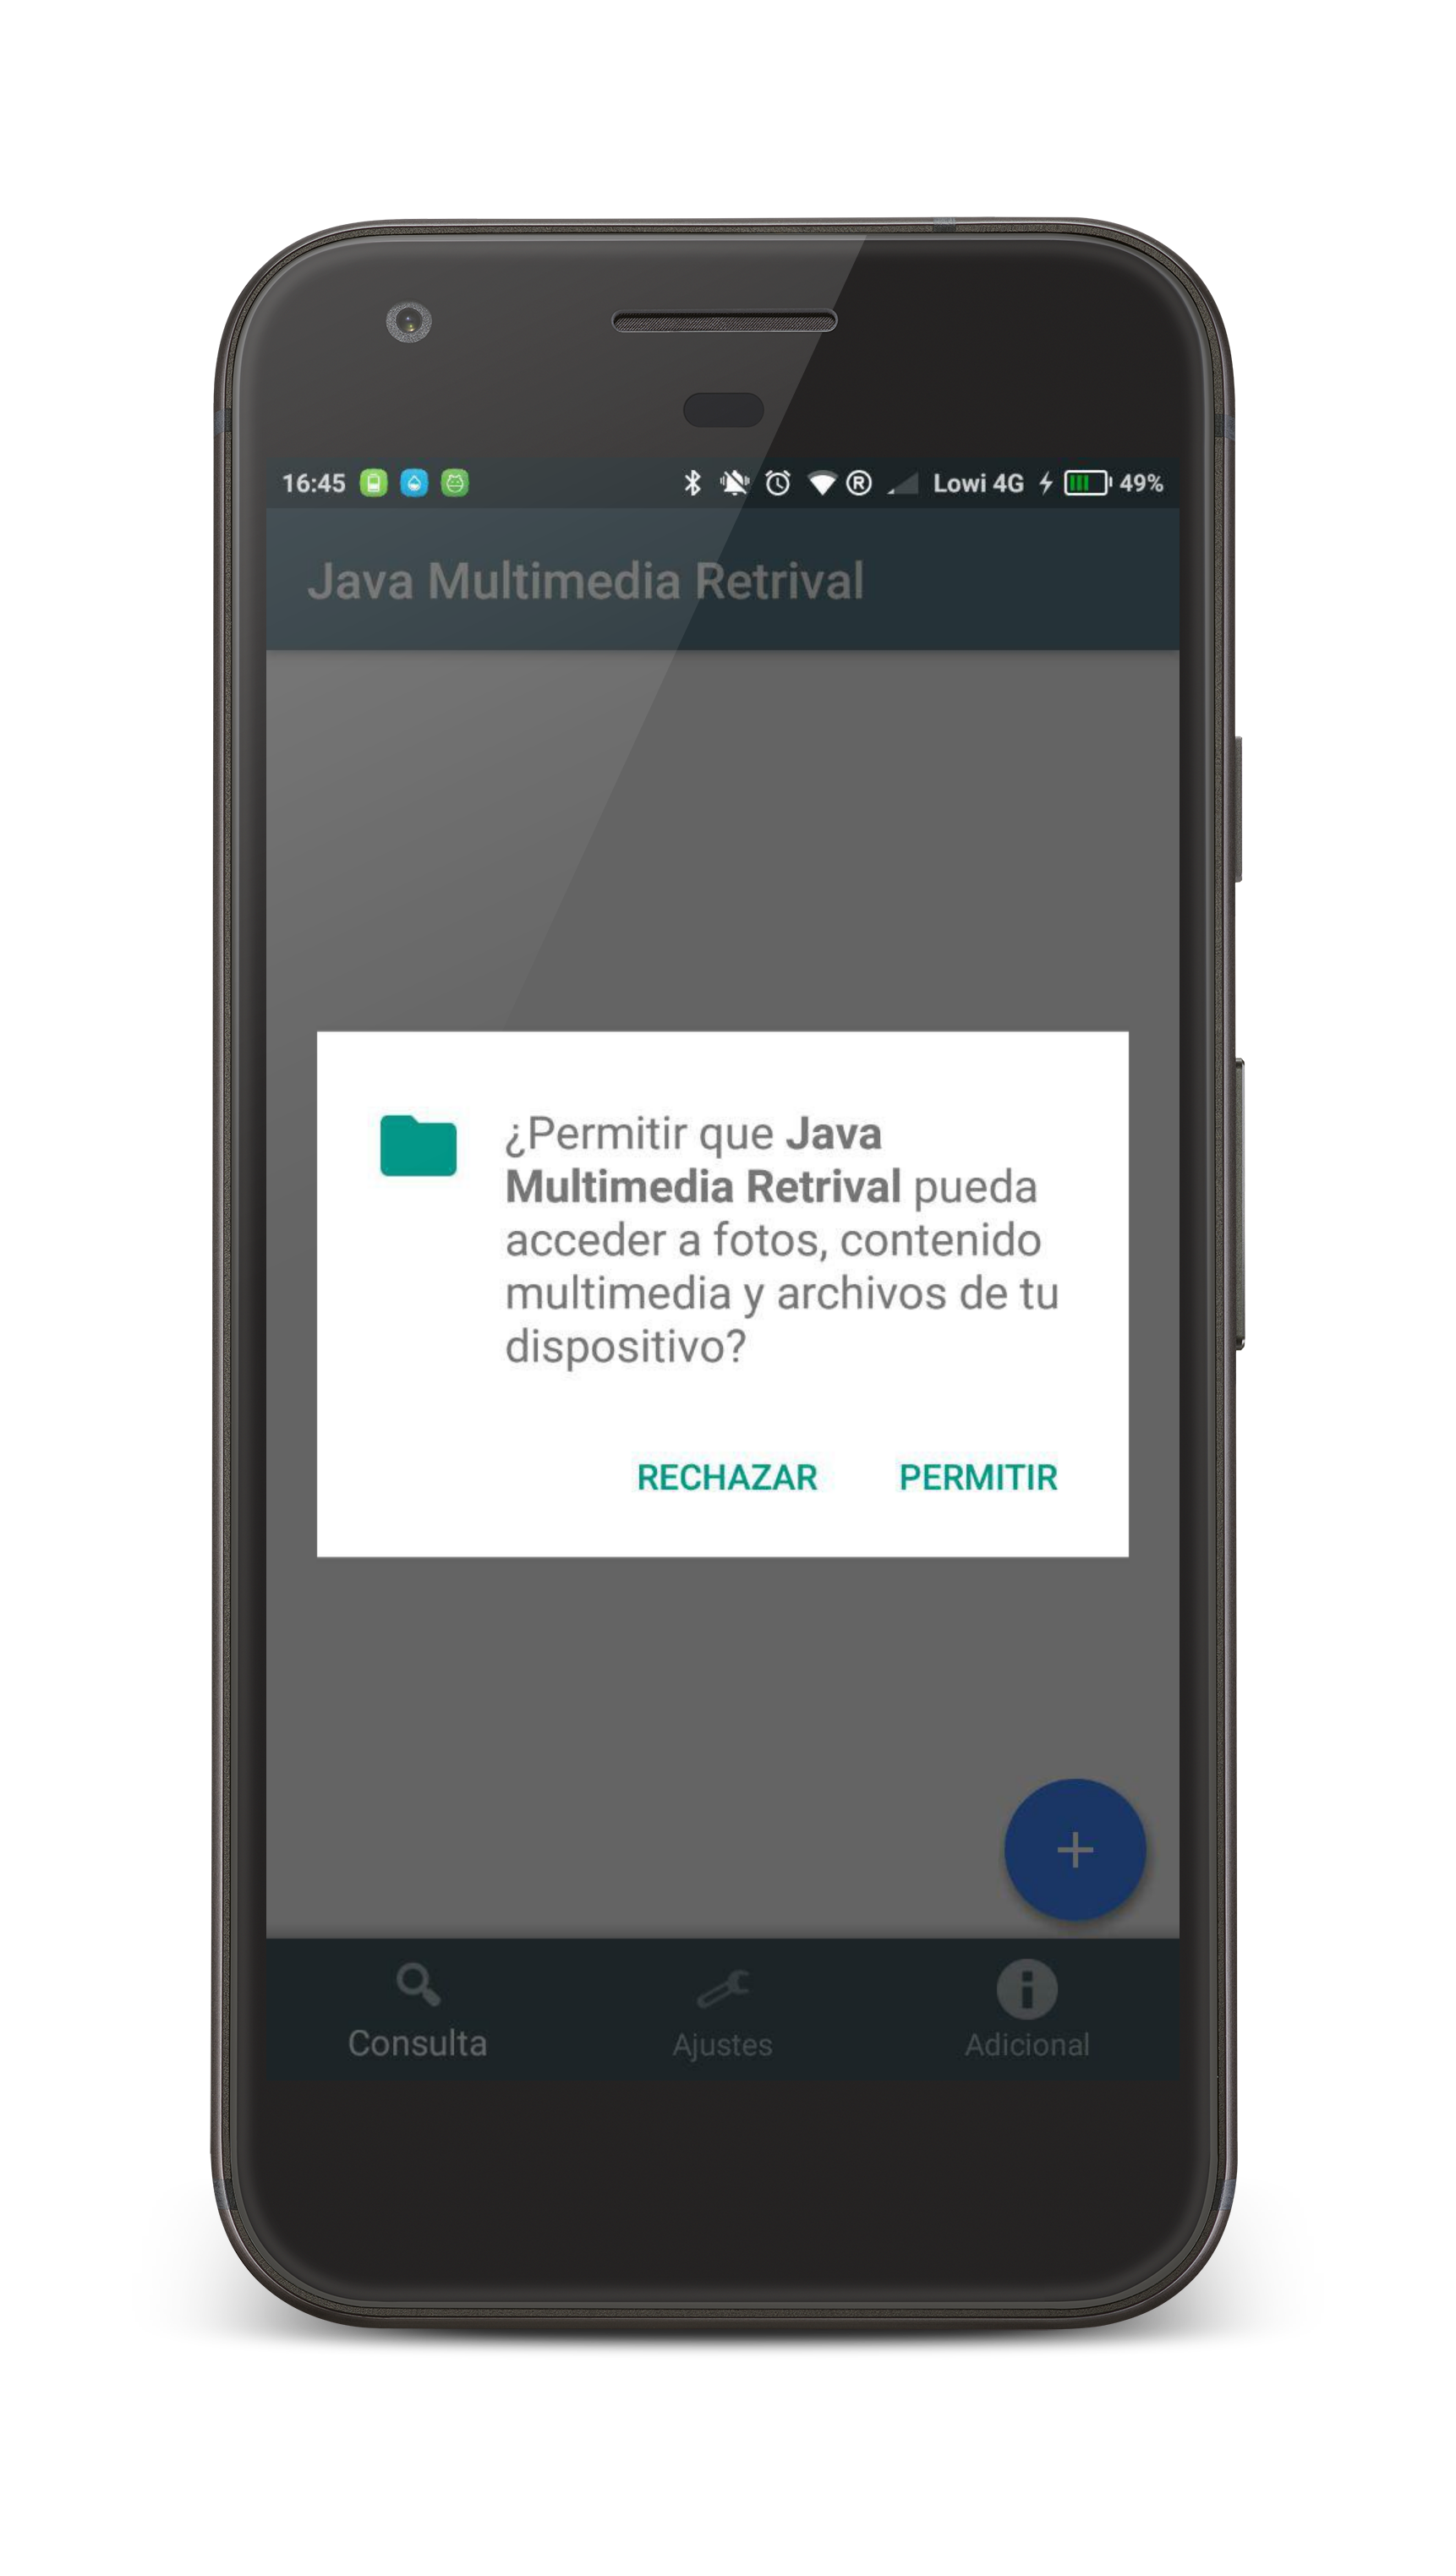
\includegraphics[scale=0.15]{imagenes/permisos1.png}  %el parámetro scale permite agrandar o achicar la imagen. En el nombre de archivo puede especificar directorios
\label{permisos1.png}
\caption{Permisos aplicación 1}
\end{figure}

En caso de no conceder el permiso, cuando intentemos acceder al recurso otra vez, galería o cámara, se nos volverá a preguntar. Una vez aceptado, ya podemos acceder a los recursos requeridos sin ningún tipo de problema.

\begin{figure}[H] %con el [H] le obligamos a situar aquí la figura
\centering
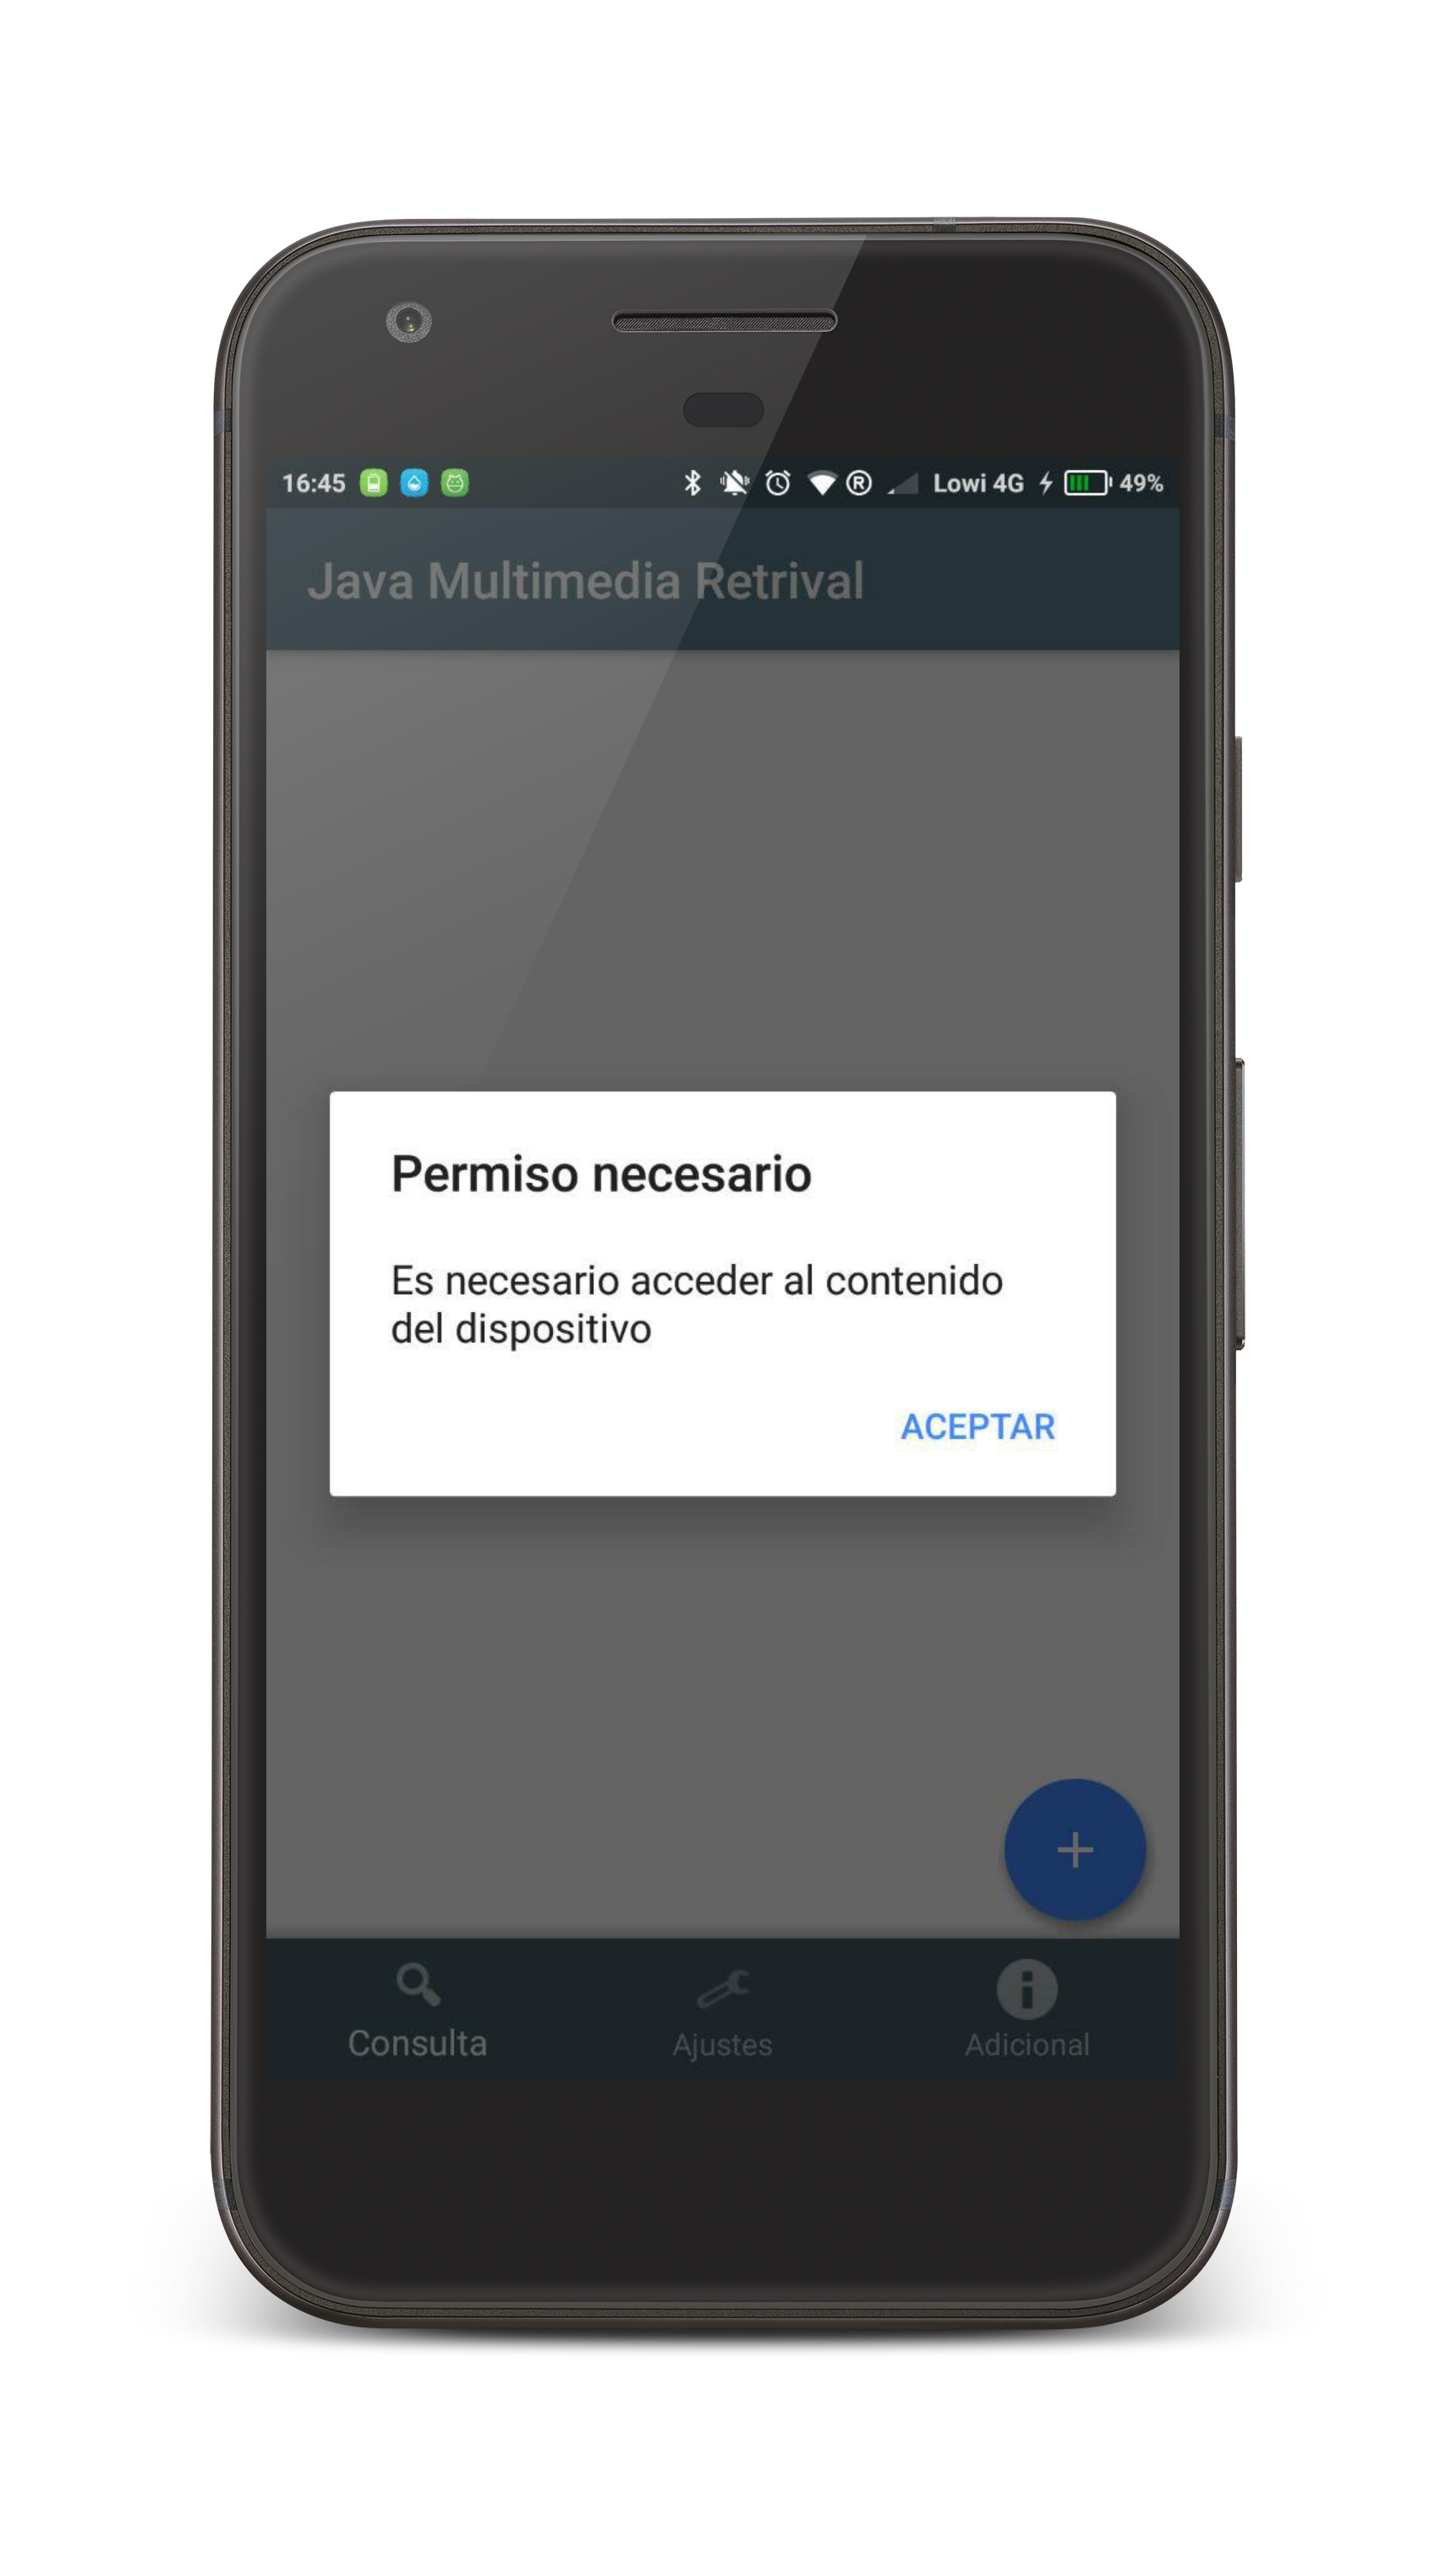
\includegraphics[scale=0.15]{imagenes/permisos2.png}  %el parámetro scale permite agrandar o achicar la imagen. En el nombre de archivo puede especificar directorios
\label{permisos2.png}
\caption{Permisos aplicación 2}
\end{figure}

\section{Navegación}

Para moverse a través de la aplicación, se dispone de un menú inferior con 3 elementos o ítems, cada uno representa una pantalla distinta. Por defecto la pantalla inicial es la correspondiente a la de consulta, ya que es el corazón de la aplicación.\\

Se pueden pulsar cada uno de los ítems para cambiar a su pantalla correspondiente. Cada pantalla tiene elementos propios y no son compartidos. Por ejemplo, el \textit{floating button} azul solo aparece en la pantalla de consulta.\\

\begin{figure}[H] %con el [H] le obligamos a situar aquí la figura
\centering
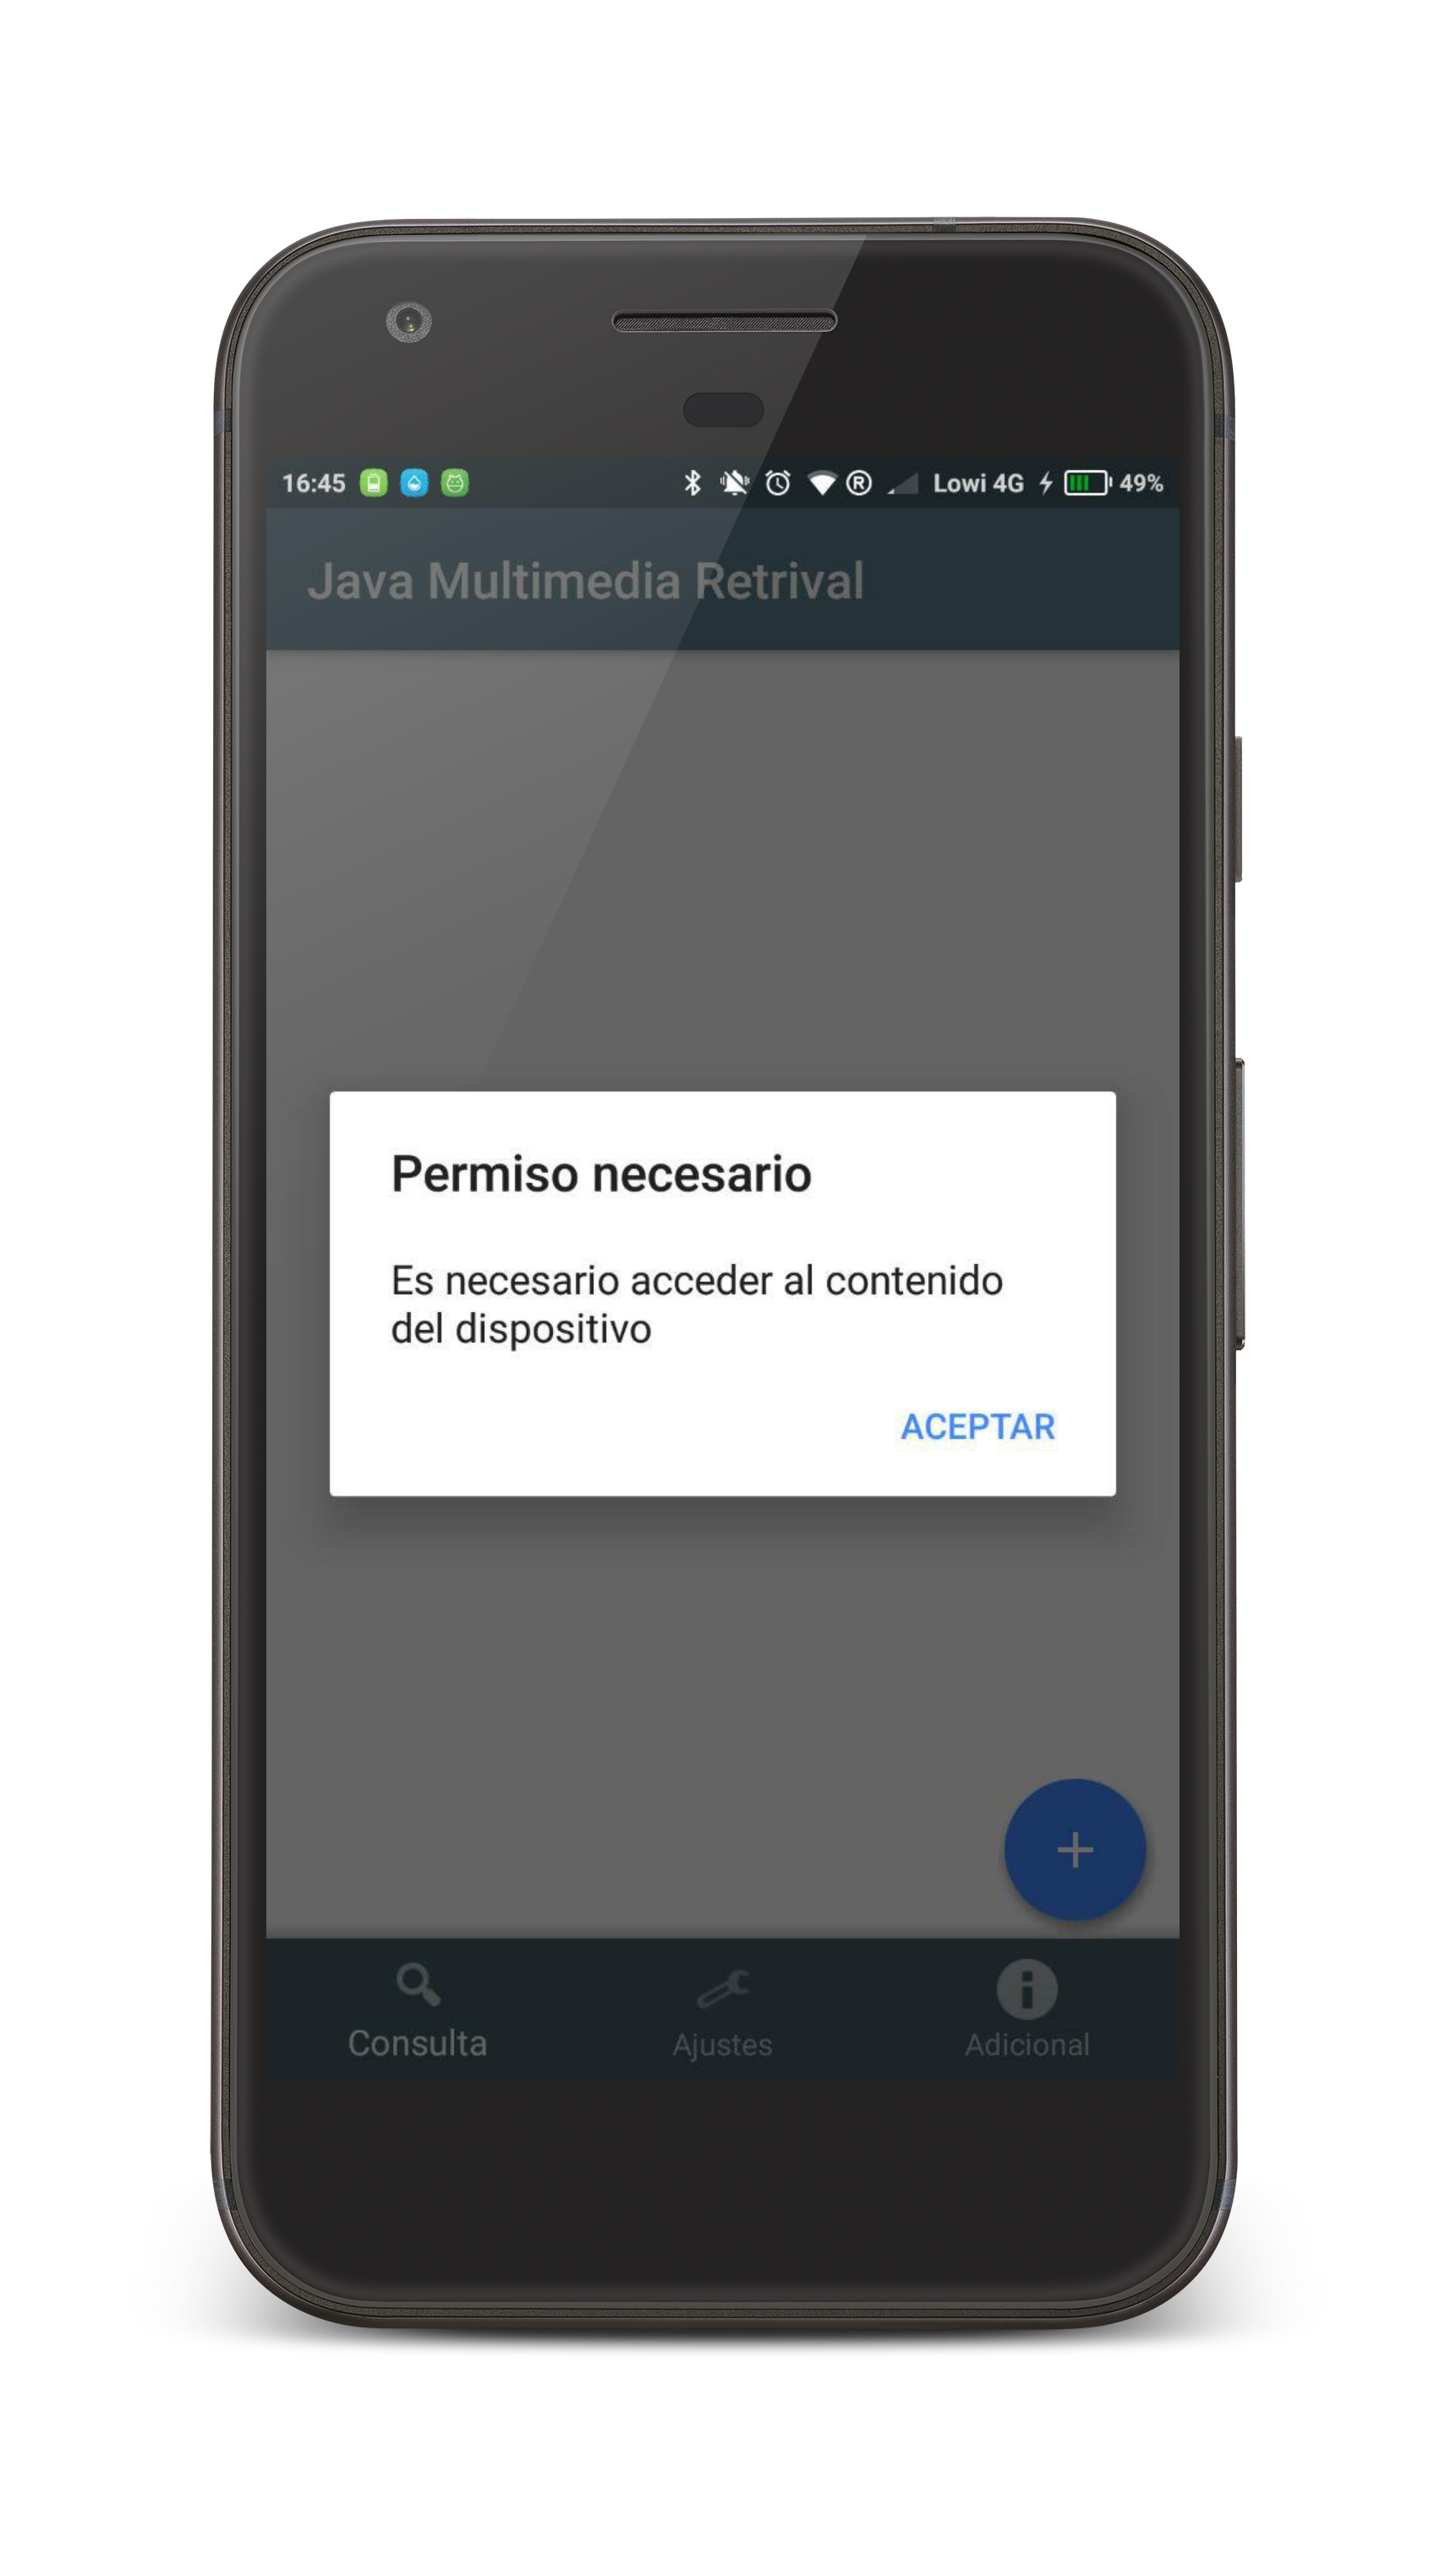
\includegraphics[scale=0.15]{imagenes/permisos2.png}  %el parámetro scale permite agrandar o achicar la imagen. En el nombre de archivo puede especificar directorios
\label{permisos2.png}
\caption{Ejemplo de navegación 1}
\end{figure}

\begin{figure}[H] %con el [H] le obligamos a situar aquí la figura
\centering
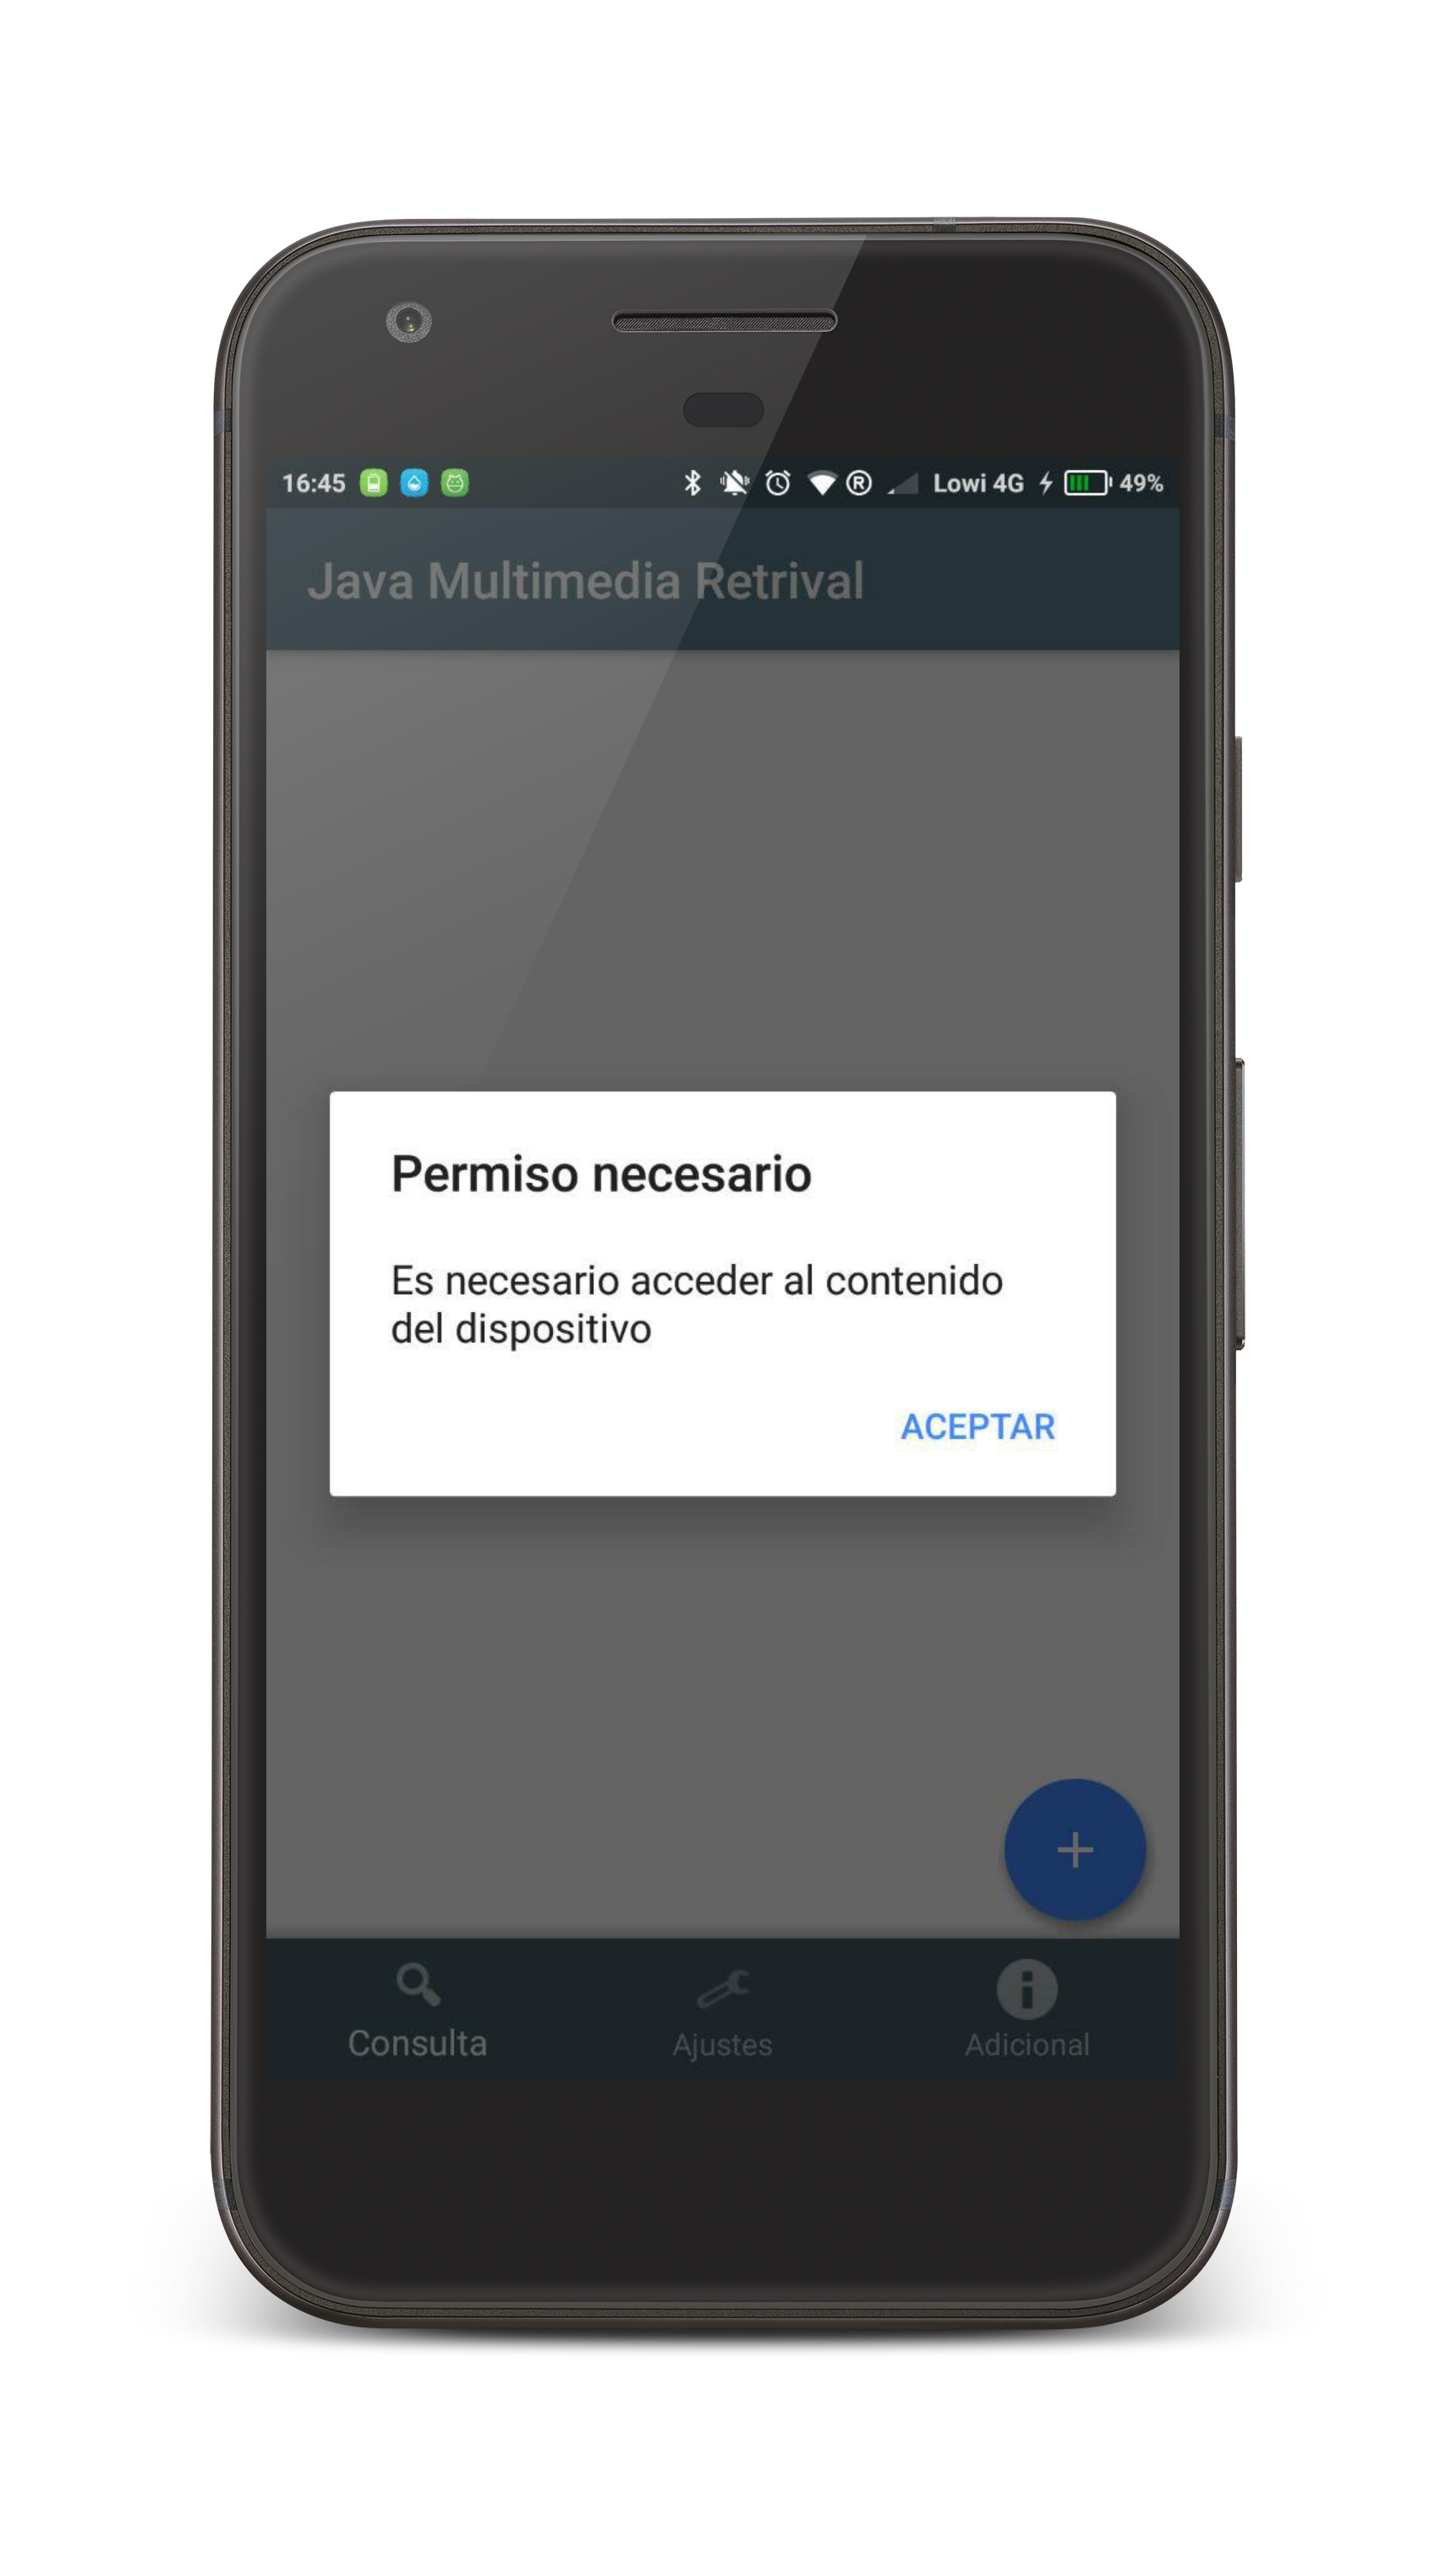
\includegraphics[scale=0.15]{imagenes/permisos2.png}  %el parámetro scale permite agrandar o achicar la imagen. En el nombre de archivo puede especificar directorios
\label{permisos2.png}
\caption{Permisos navegación 2}
\end{figure}

\section{Consulta}

Para realizar la consulta disponemos de dos opciones, elegir una imagen desde la cámara o desde la galería. Estas opciones aparecen al pulsar sobre el botón flotante. Una vez elegida una, se lanzará la cámara, pudiendo elegir la trasera o delantera, o la galería, mediante la cual podremos acceder a cualquier imagen del dispositivo. Cuando sea seleccionada, esta aparecerá en la parte superior de la aplicación.

\begin{figure}[H] %con el [H] le obligamos a situar aquí la figura
\centering
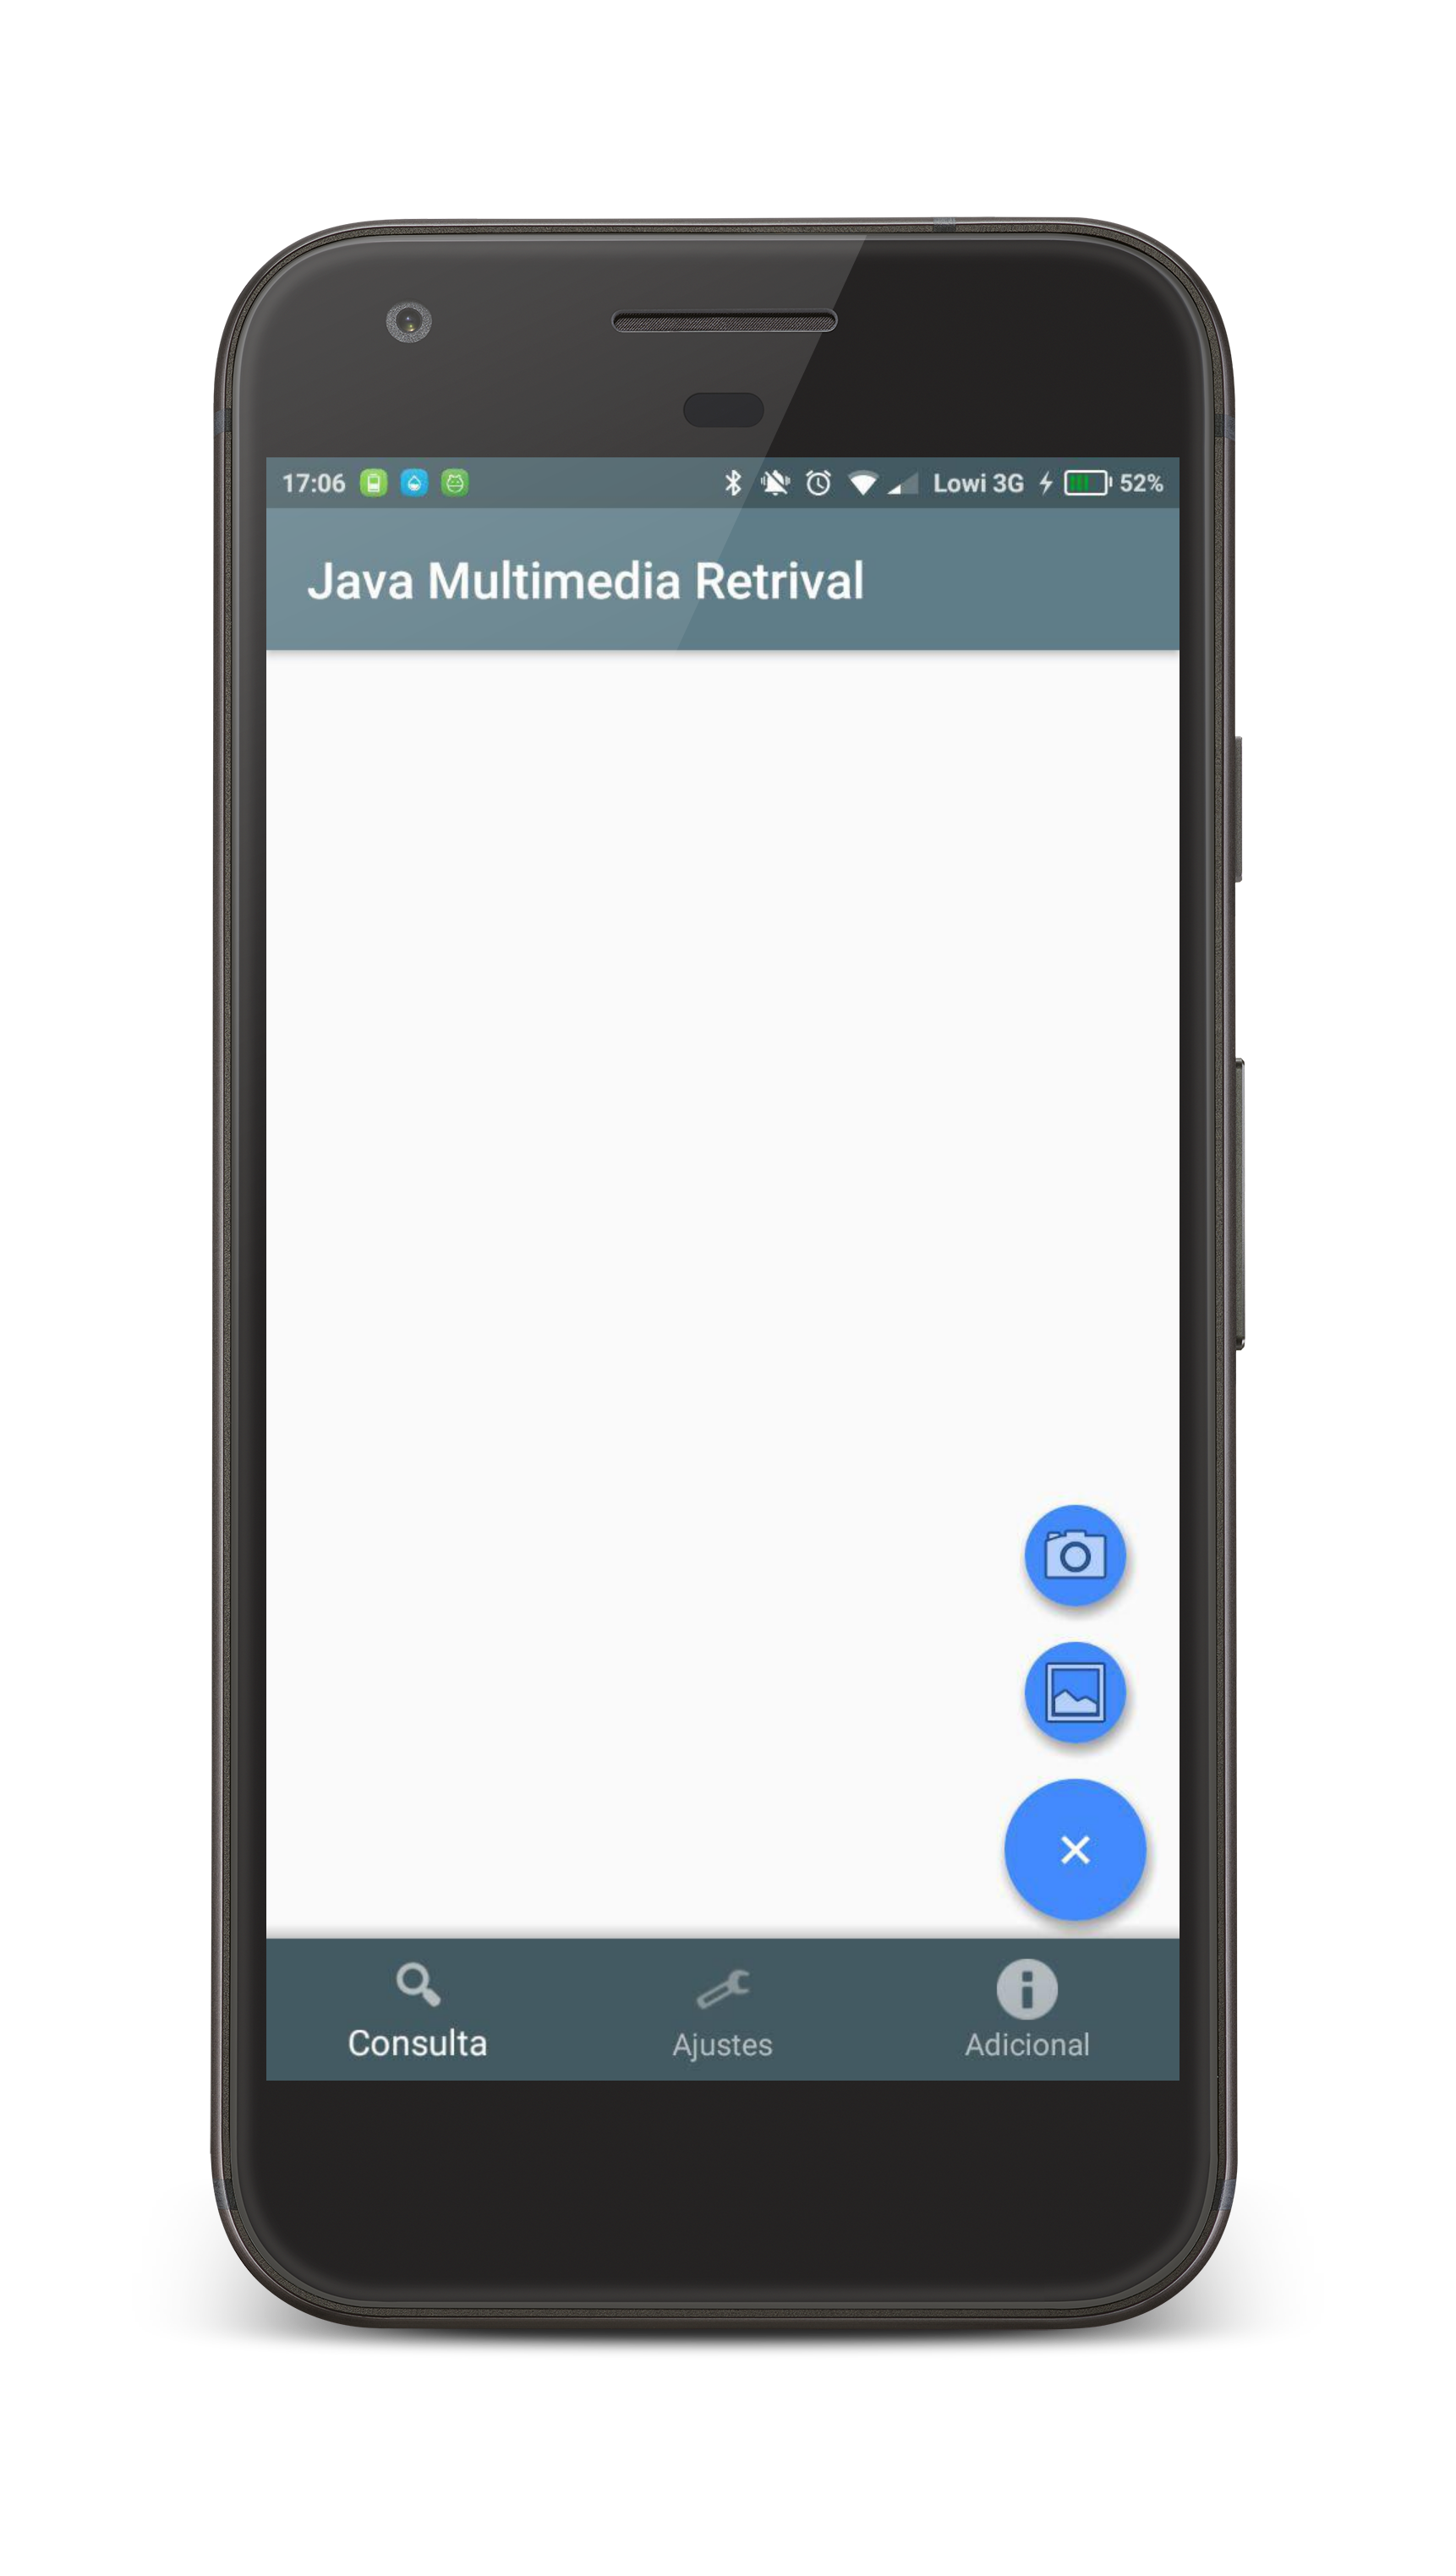
\includegraphics[scale=0.15]{imagenes/hacerconsulta.png}  %el parámetro scale permite agrandar o achicar la imagen. En el nombre de archivo puede especificar directorios
\label{hacerconsulta.png}
\caption{Realizar consulta}
\end{figure}

\section{Ajustes}

En este apartado vamos a hablar de los ajustes que puede realizar el usuario sobre las consultas.\\

\begin{figure}[H] %con el [H] le obligamos a situar aquí la figura
\centering
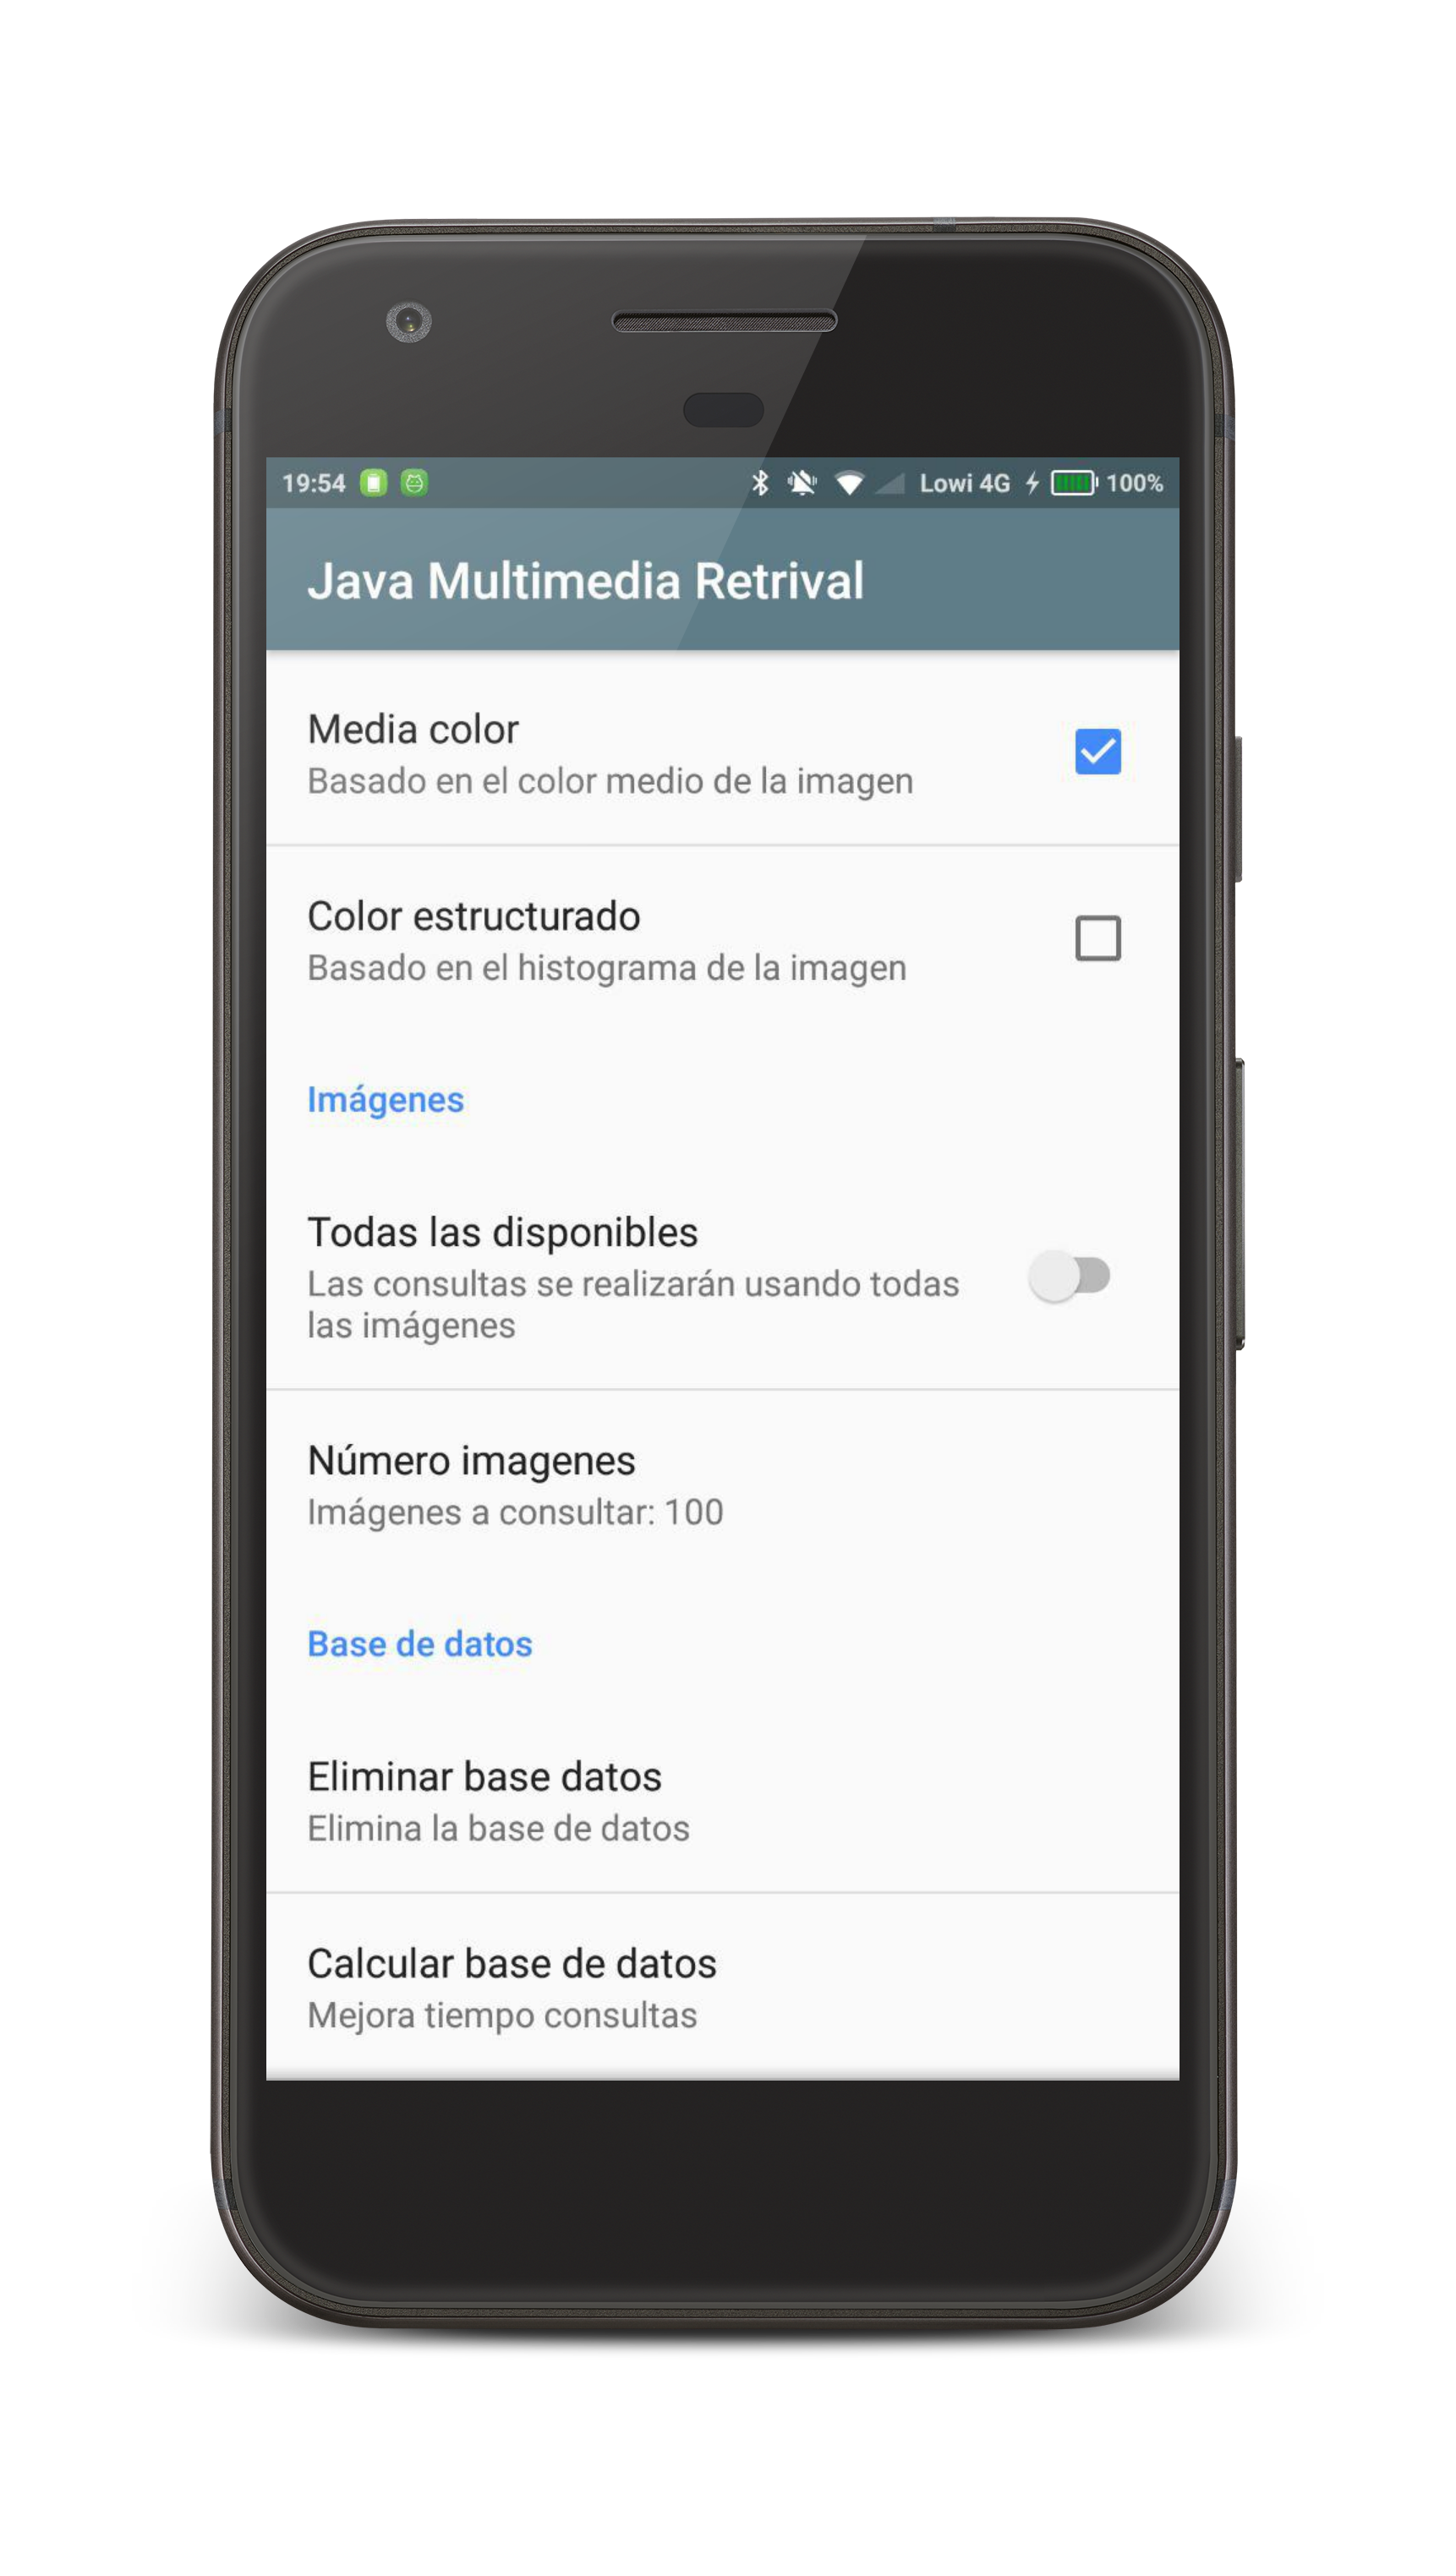
\includegraphics[scale=0.15]{imagenes/ajustes.png}  %el parámetro scale permite agrandar o achicar la imagen. En el nombre de archivo puede especificar directorios
\label{ajustes.png}
\caption{Pantalla ajustes}
\end{figure}

Podríamos hablar de tres secciones:

\subsection{Descriptores}

Aquí podemos encontrar los descriptores de los que dispone la aplicación. El usuario puede elegir uno libremente, pero solo un descriptor puede ser elegido a la vez.

\begin{figure}[H] %con el [H] le obligamos a situar aquí la figura
\centering

\includegraphics[scale=0.5]{imagenes/ajustesdescriptor.png}  %el parámetro scale permite agrandar o achicar la imagen. En el nombre de archivo puede especificar directorios
\label{ajustesdescriptor.png}
\caption{Pantalla ajustes. Sección descriptores}
\end{figure}

\subsection{Imágenes}

En este apartado el usuario puede elegir el número de imágenes totales sobre las cuales quiere realizar la consulta. Tiene dos opciones, introducir dicho valor manualmente o seleccionar todas las del dispositivo. Este valor también se usa en el caso de querer calcular la base de datos, cosa que veremos a continuación.

\begin{figure}[H] %con el [H] le obligamos a situar aquí la figura
\centering
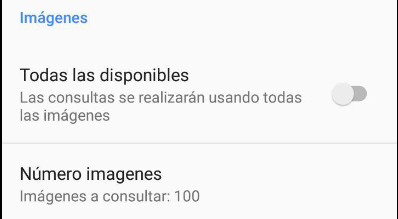
\includegraphics[scale=0.5]{imagenes/ajustesimagenes.png}  %el parámetro scale permite agrandar o achicar la imagen. En el nombre de archivo puede especificar directorios
\label{ajustesimagenes.png}
\caption{Pantalla ajustes. Sección imágenes}
\end{figure}

\subsection{Base de datos}

Aquí el usuario puede precalcular la base de datos, de esta manera al realizar la consulta no se calcularán nada, simplemente se obtendrán los valores de la base de datos. Este precálculo se realiza para todos los descriptores del sistema.\\

Por otro lado, puede borrar la base de datos si así lo desea. Realizando se calcularán los valores de la base de datos durante la consulta.

\begin{figure}[H] %con el [H] le obligamos a situar aquí la figura
\centering
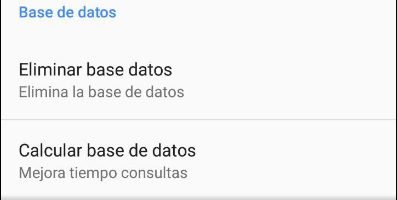
\includegraphics[scale=0.5]{imagenes/ajustesbd.png}  %el parámetro scale permite agrandar o achicar la imagen. En el nombre de archivo puede especificar directorios
\label{ajustesbd.png}
\caption{Pantalla ajustes. Sección base de datos}
\end{figure}

\section{Adicional}

En esta sección el usuario puede encontrar información relacionada con el proyecto, así como sobre su desarrollador. Al pulsar en cualquier opción esta le llevará a su correspondiente página web con una mayor cantidad de información.\\

Debido a que este tipo de sistema, \textit{CBIR}, no es muy conocido por los usuarios, al igual que los descriptores, se proporciona una serie de enlaces con información básica sobre ellos, en caso de que el usuario quiera aprender más o sienta curiosidad sobre el tema.

\begin{figure}[H] %con el [H] le obligamos a situar aquí la figura
\centering
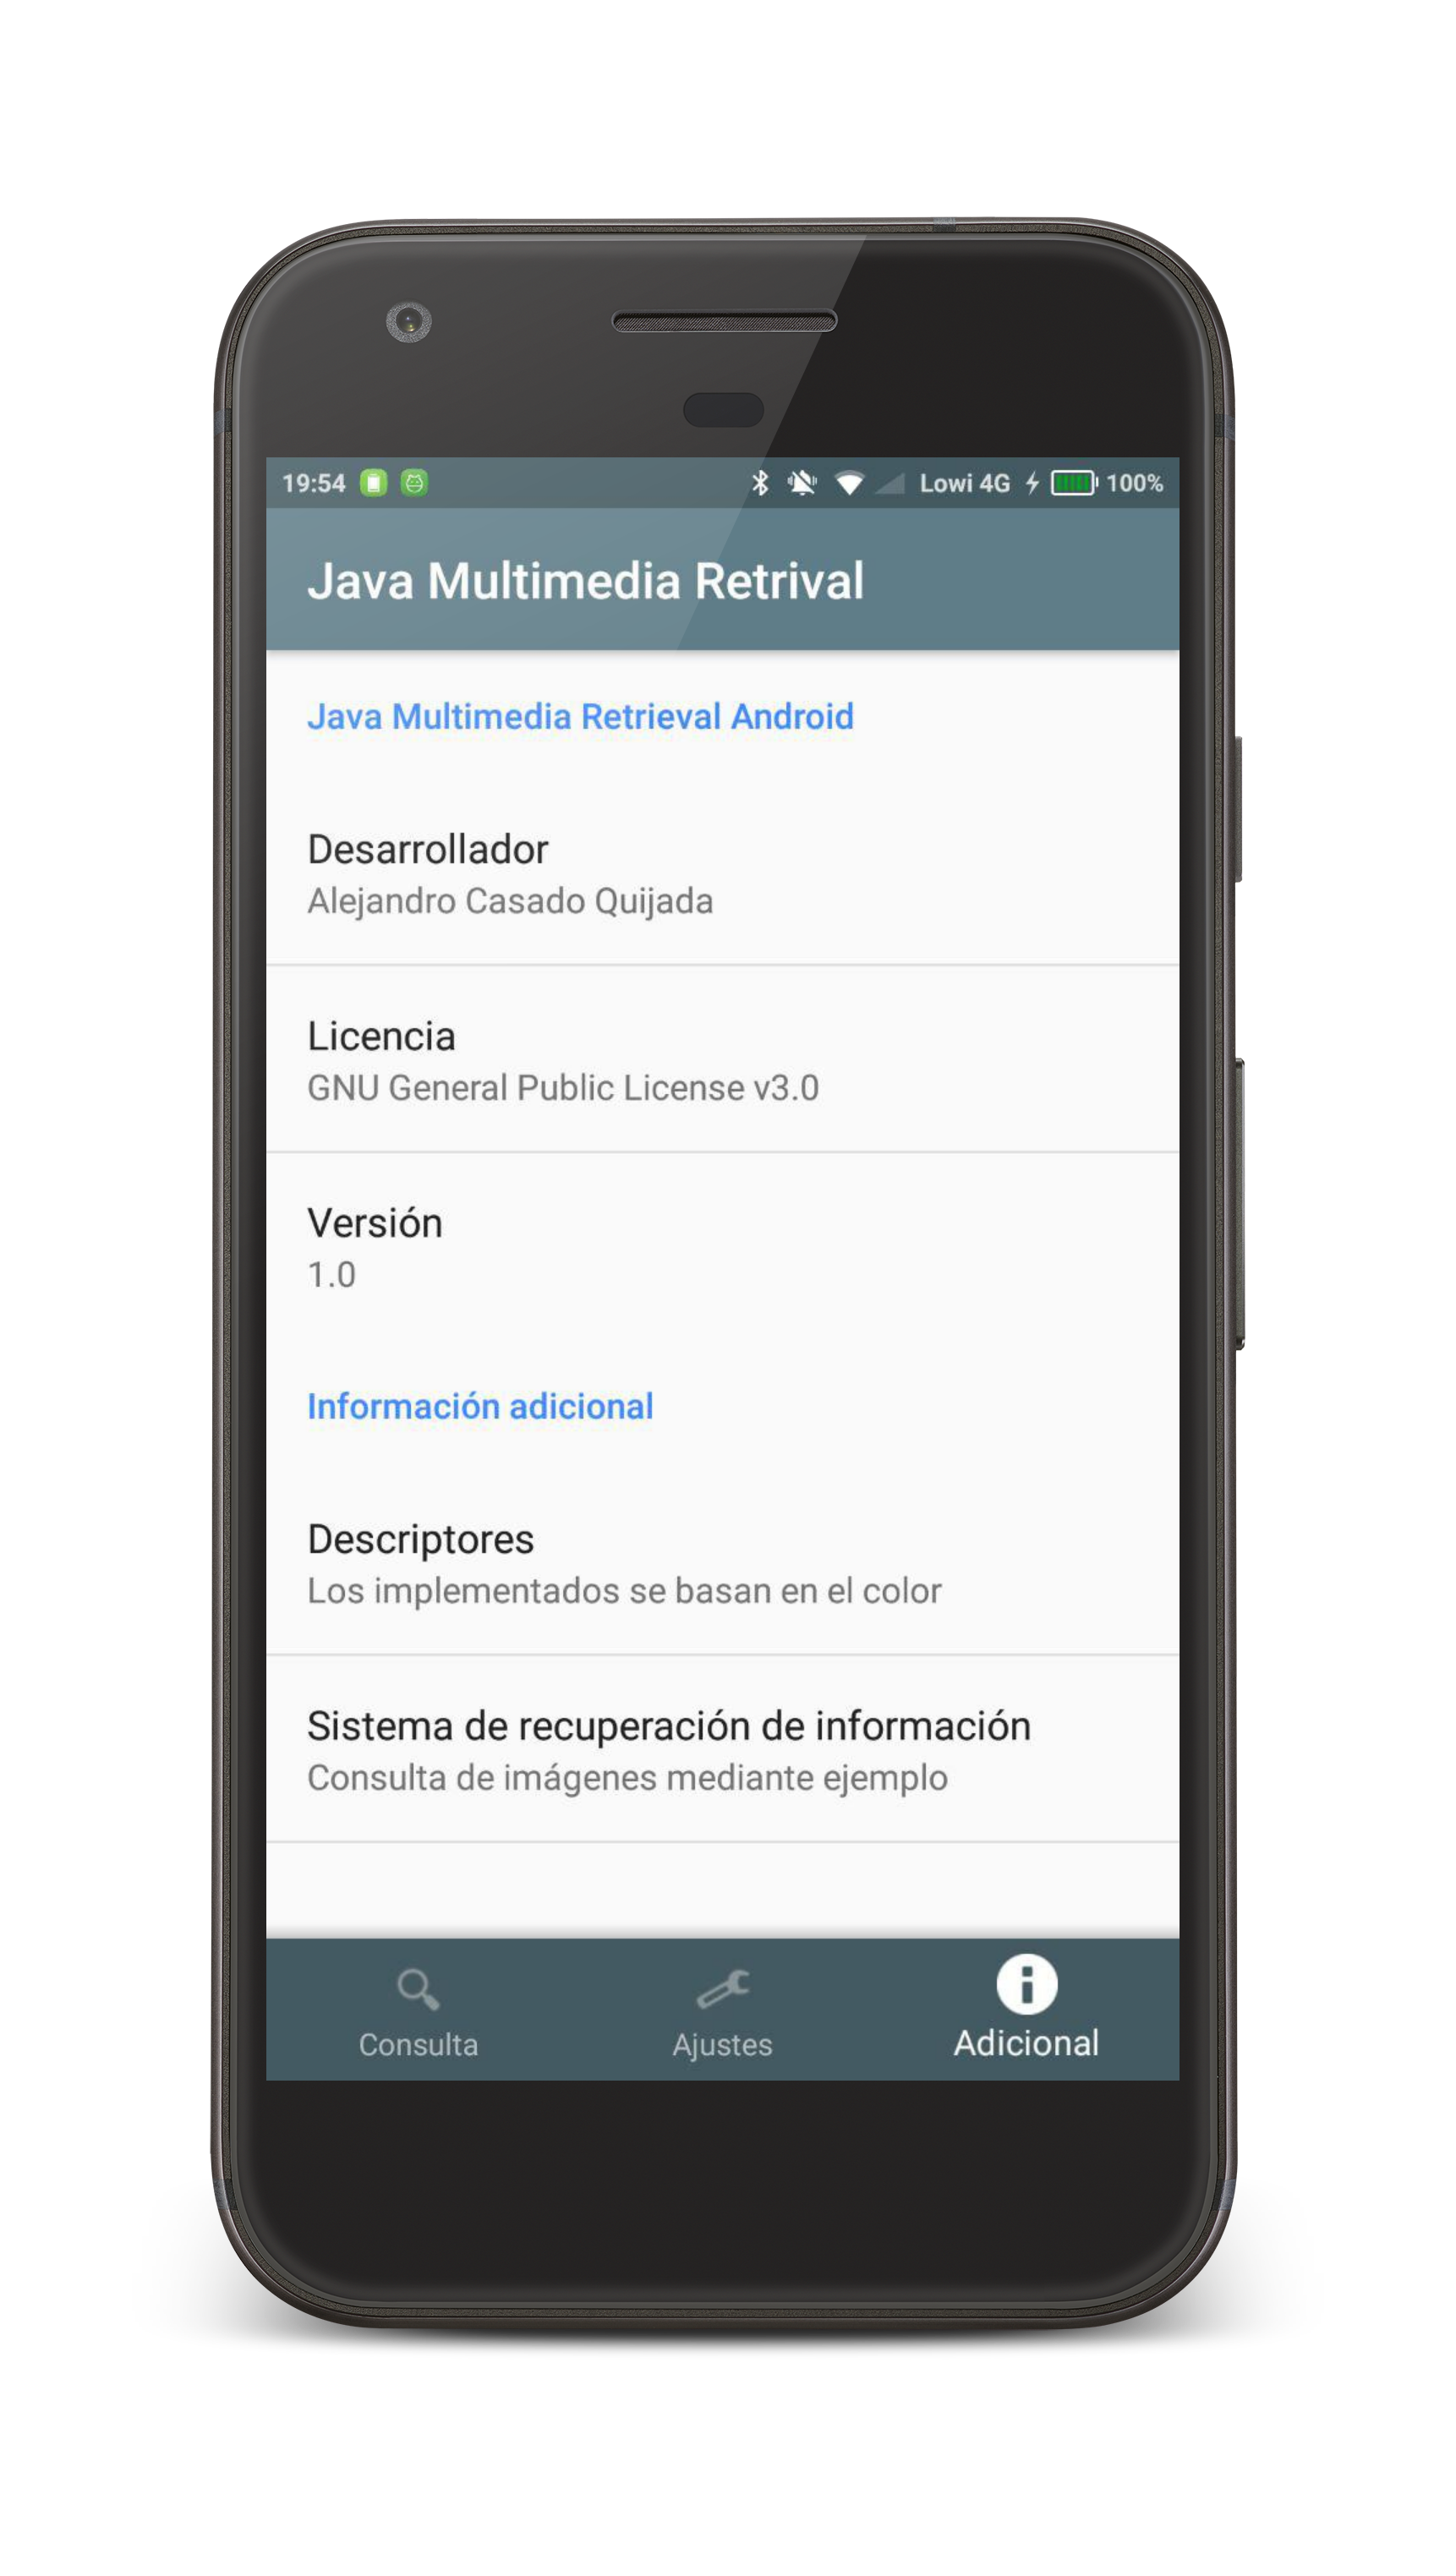
\includegraphics[scale=0.15]{imagenes/adicional.png}  %el parámetro scale permite agrandar o achicar la imagen. En el nombre de archivo puede especificar directorios
\label{adicional.png}
\caption{Pantalla adicional}
\end{figure}









%\input{apendices/licencia/licencia}
%%\input{apendices/paper/paper}
%\input{glosario/entradas_glosario}
% \addcontentsline{toc}{chapter}{Glosario}
% \printglossary
%\chapter*{}
\thispagestyle{empty}

\end{document}
